% ========================================================
% FILE: sections/3.Software_Requirement_Specification.tex
% Part III: Software Requirement Specification (Executive format matching docs_NA)
% ========================================================
\part{Software Requirement Specification}

\section{System Actors}

The \textbf{Frevia} platform operates as a multi-role ecosystem involving five primary human stakeholder roles alongside core automated system and external service actors (Figure~\ref{fig:context-diagram} and Table~\ref{tab:srs_actors}). Unauthenticated visitors (Guests) may only browse public marketplace listings and initiate account onboarding, whereas authenticated roles operate within strictly isolated RBAC boundaries.

\begin{figure}[H]
    \centering
    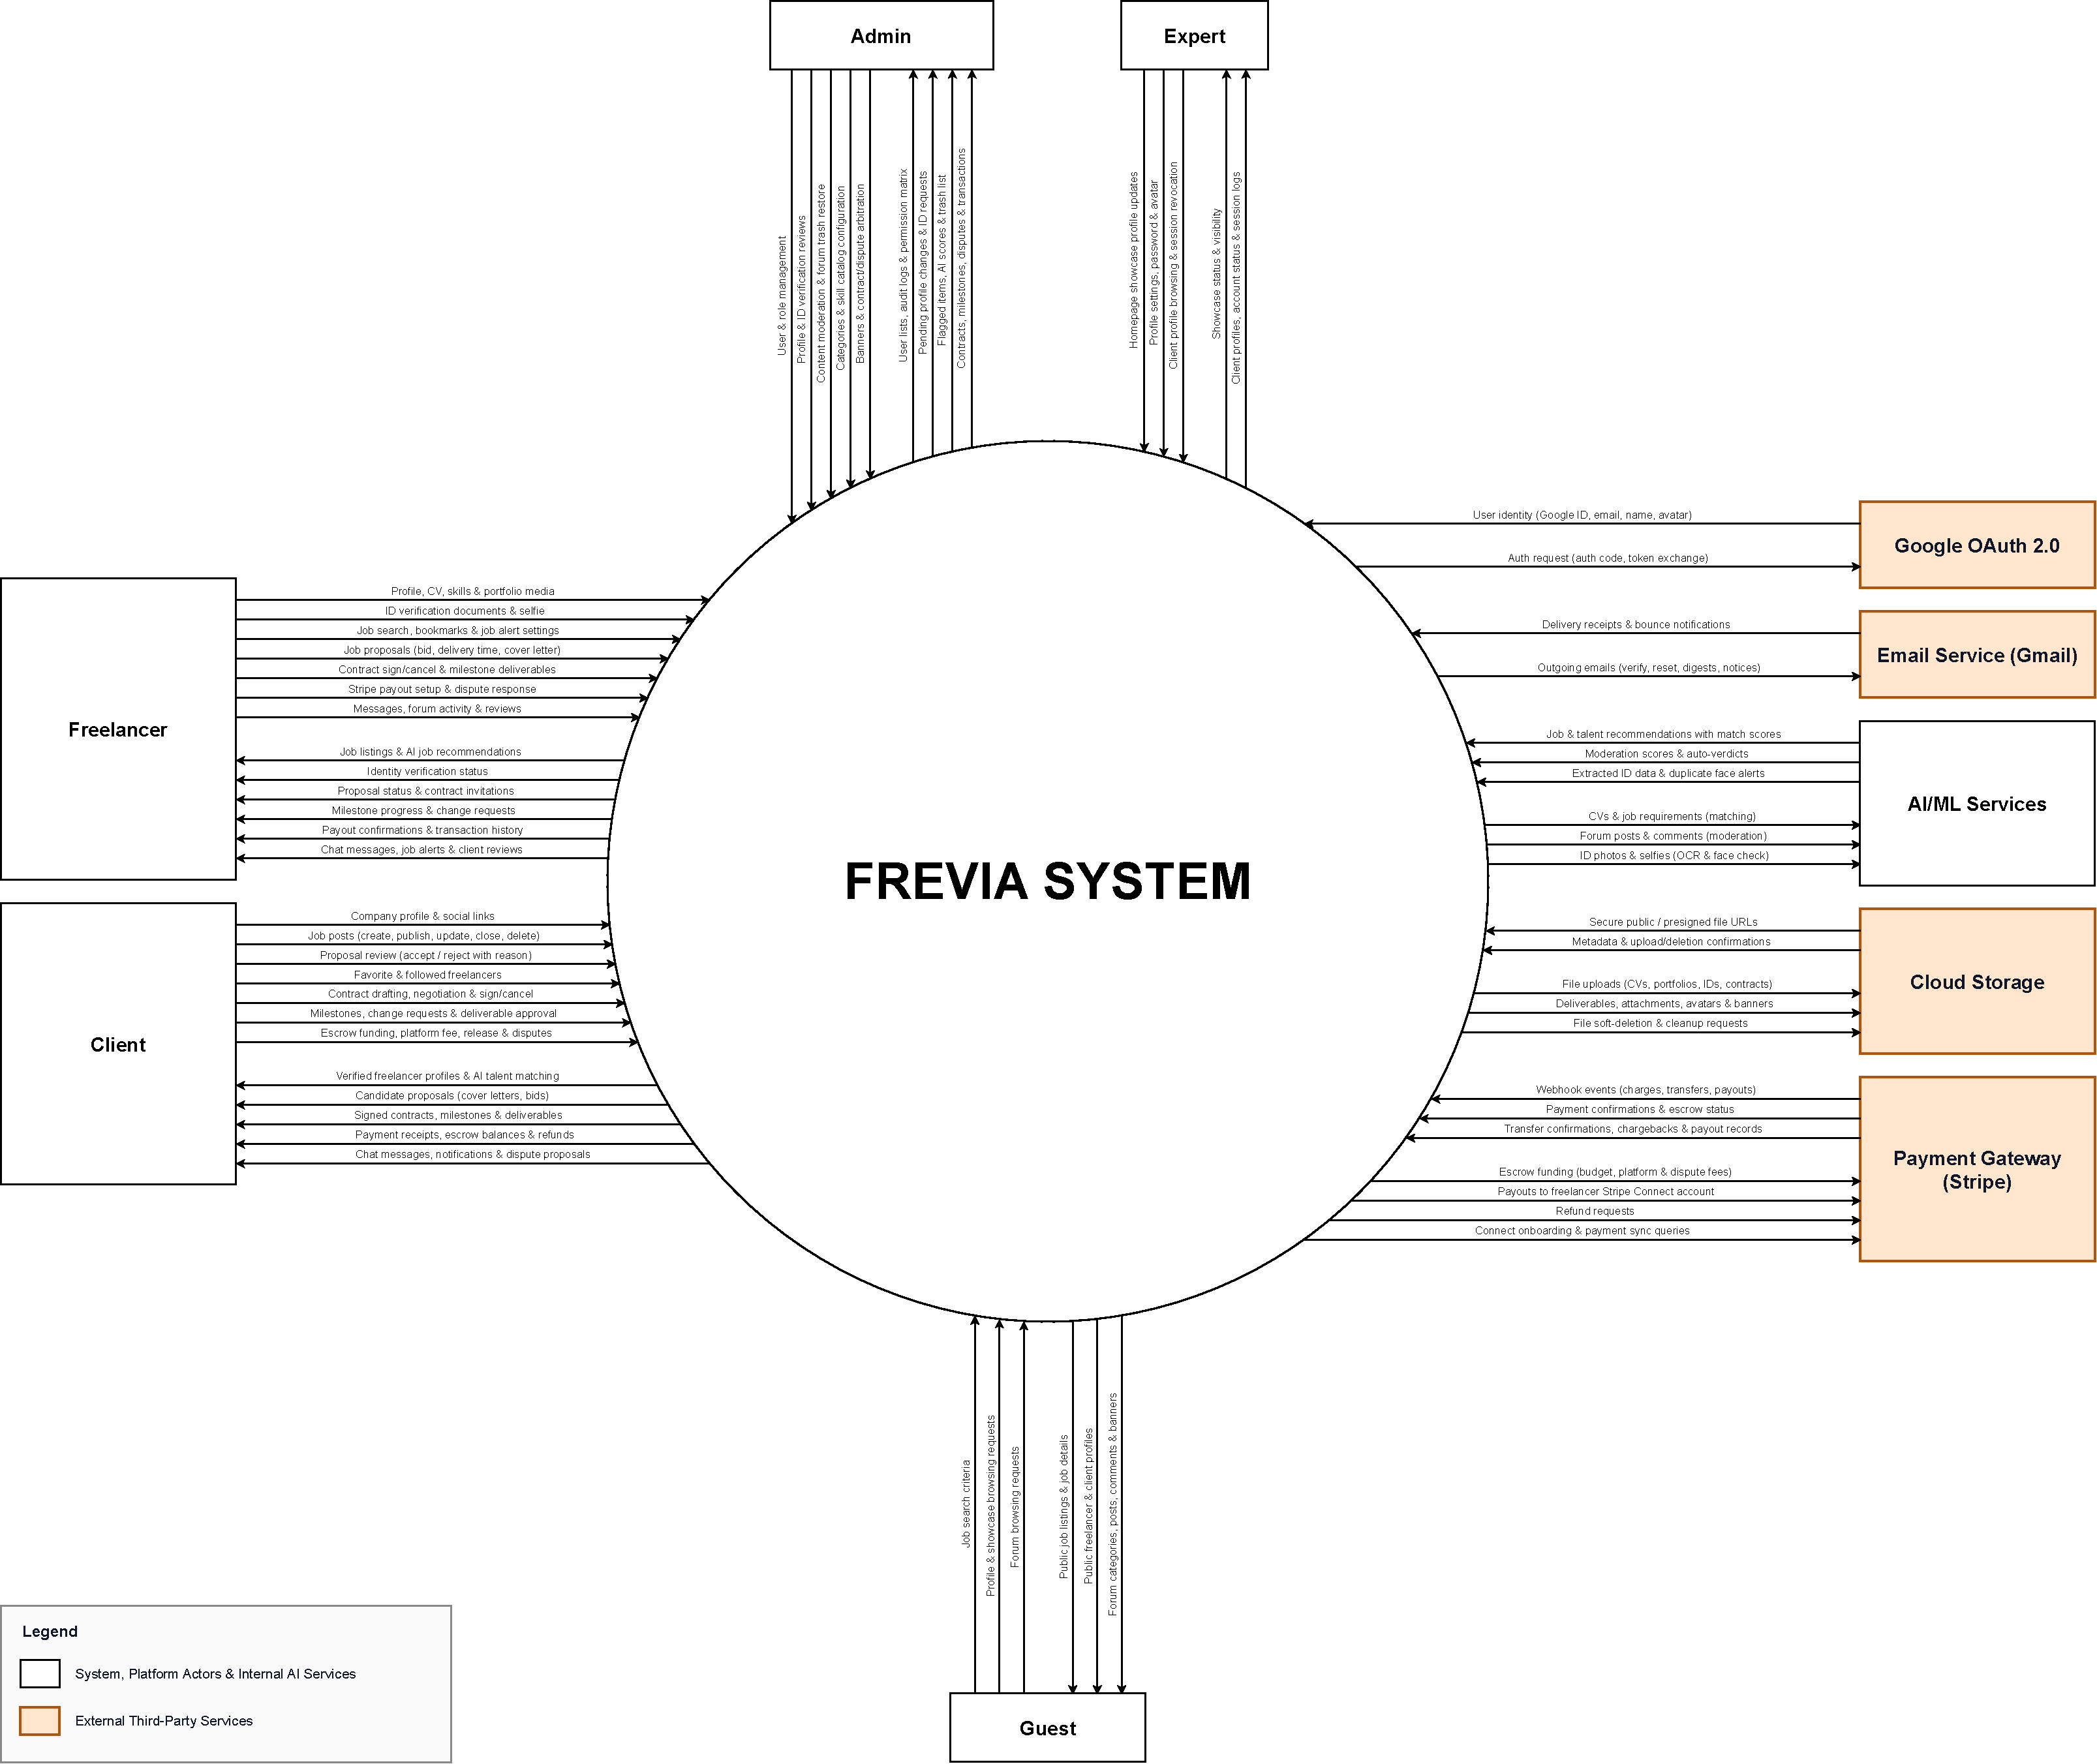
\includegraphics[width=0.88\linewidth,height=0.68\textheight,keepaspectratio]{image/context_diagram/context-diagram.pdf}
    \caption{Frevia System Context Diagram}
    \label{fig:context-diagram}
\end{figure}

\begingroup
\renewcommand{\arraystretch}{1.35}
\small
\setlength{\tabcolsep}{5pt}
\begin{longtable}{|C{0.9cm}|L{3.5cm}|L{10.2cm}|}
\caption{Actors of the Frevia Platform}\label{tab:srs_actors} \\
\hline
\rowcolor{fptHeader}
\textbf{No} & \textbf{Actor} & \textbf{Description} \\ \hline
\endfirsthead
\hline
\rowcolor{fptHeader}
\textbf{No} & \textbf{Actor} & \textbf{Description} \\ \hline
\endhead
\hline\endfoot
\hline\endlastfoot
1 & Guest & Unregistered visitor browsing public job postings, freelancer profiles, portfolios, and community forum posts; can register with email OTP or Google OAuth and sign in. \\ \hline
2 & Client & Individual or organization publishing fixed-price job postings, evaluating AI-ranked proposals, hiring talent, signing bilateral contracts, funding Stripe milestone escrow, reviewing deliverables, filing/responding to disputes, and submitting reviews. \\ \hline
3 & Freelancer & Service provider managing specialized profiles, skills, portfolios, CV AI parsing, and eKYC verification; searching/applying for jobs, signing contracts, uploading shared/milestone deliverables, contesting disputes, and receiving Stripe Connect payouts. \\ \hline
4 & Expert & Verified senior specialist featured in the public expert showcase who manages expert credentials and adjudicates escalated milestone disputes to issue binding escrow split rulings. \\ \hline
5 & Administrator & Internal platform operator overseeing RBAC roles and route permissions, active user accounts, eKYC identity verification audits, forum content moderation, system catalogs, banners, and administrative dispute arbitration. \\ \hline
6 & Automated System & Background scheduler and state engine handling proposal/contract expirations, dispute response deadlines, automated notification dispatches, and ledger reconciliation. \\ \hline
7 & External Integrations & Supporting microservices and third-party providers: FastAPI AI microservices (\texttt{cv-matching}, \texttt{id-verification}, optional \texttt{ai-moderation}), \textbf{Stripe} (Checkout \& Connect Express), \textbf{Cloudinary} CDN, \textbf{Google OAuth 2.0}, and \textbf{SMTP}. \\ \hline
\end{longtable}
\endgroup

\section{Use Case Diagram}

Figures~\ref{fig:uc_guest_1} through \ref{fig:uc_admin_4} organize all functional use cases across every stakeholder role (\textbf{Guest}, \textbf{Client}, \textbf{Freelancer}, \textbf{Expert}, and \textbf{Administrator}), illustrating clear permission separation and workflow groupings.

% =========================================================================
% 1. Guest Use Case Diagram
% =========================================================================
\begin{figure}[H]
    \centering
    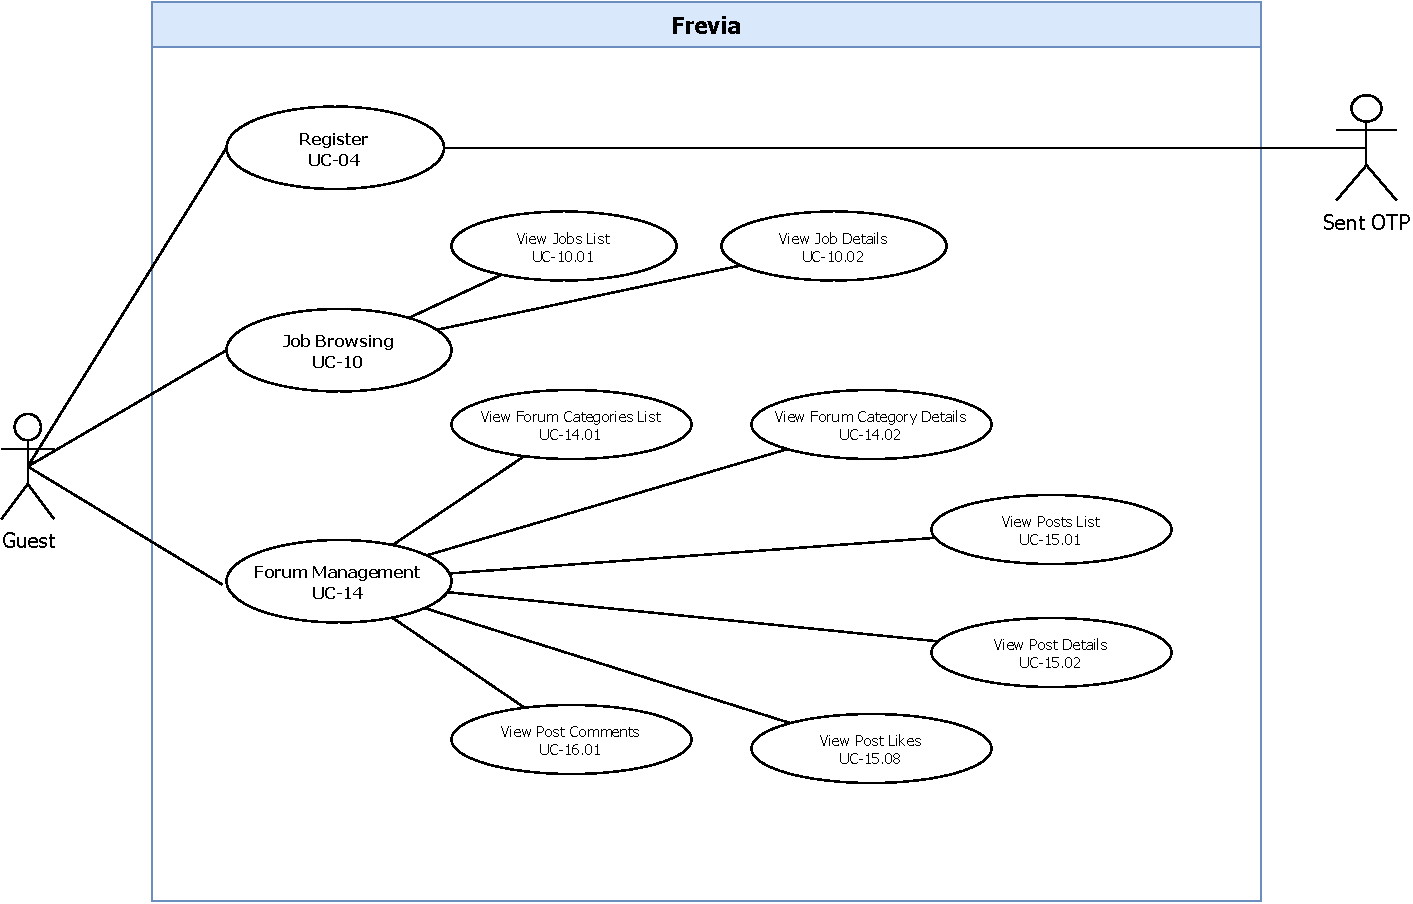
\includegraphics[
        width=\textwidth,
        height=0.85\textheight,
        keepaspectratio
    ]{image/UC_diagram/Guest.pdf}
    \caption{Guest Usecase}
    \label{fig:uc_guest_1}
\end{figure}

% =========================================================================
% 2. Client Use Case Diagrams
% =========================================================================
\begin{figure}[H]
    \centering
    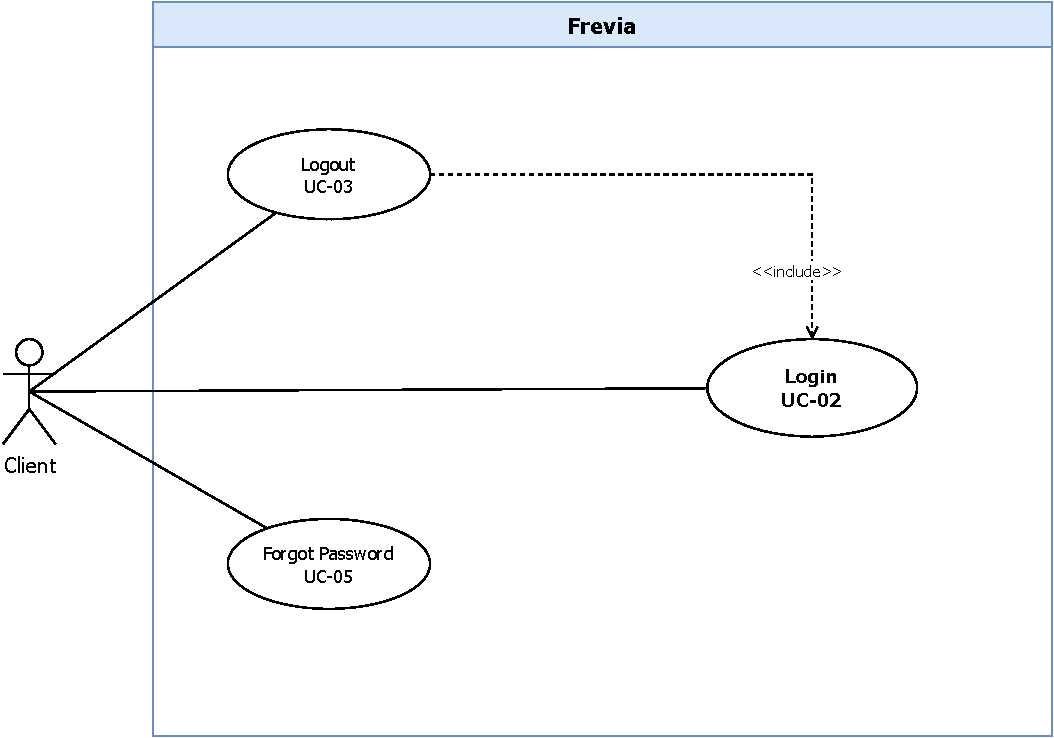
\includegraphics[
        width=\textwidth,
        height=0.85\textheight,
        keepaspectratio
    ]{image/UC_diagram/Client_1.pdf}
    \caption{Client Usecase 1/6}
    \label{fig:uc_client_1}
\end{figure}

\begin{figure}[H]
    \centering
    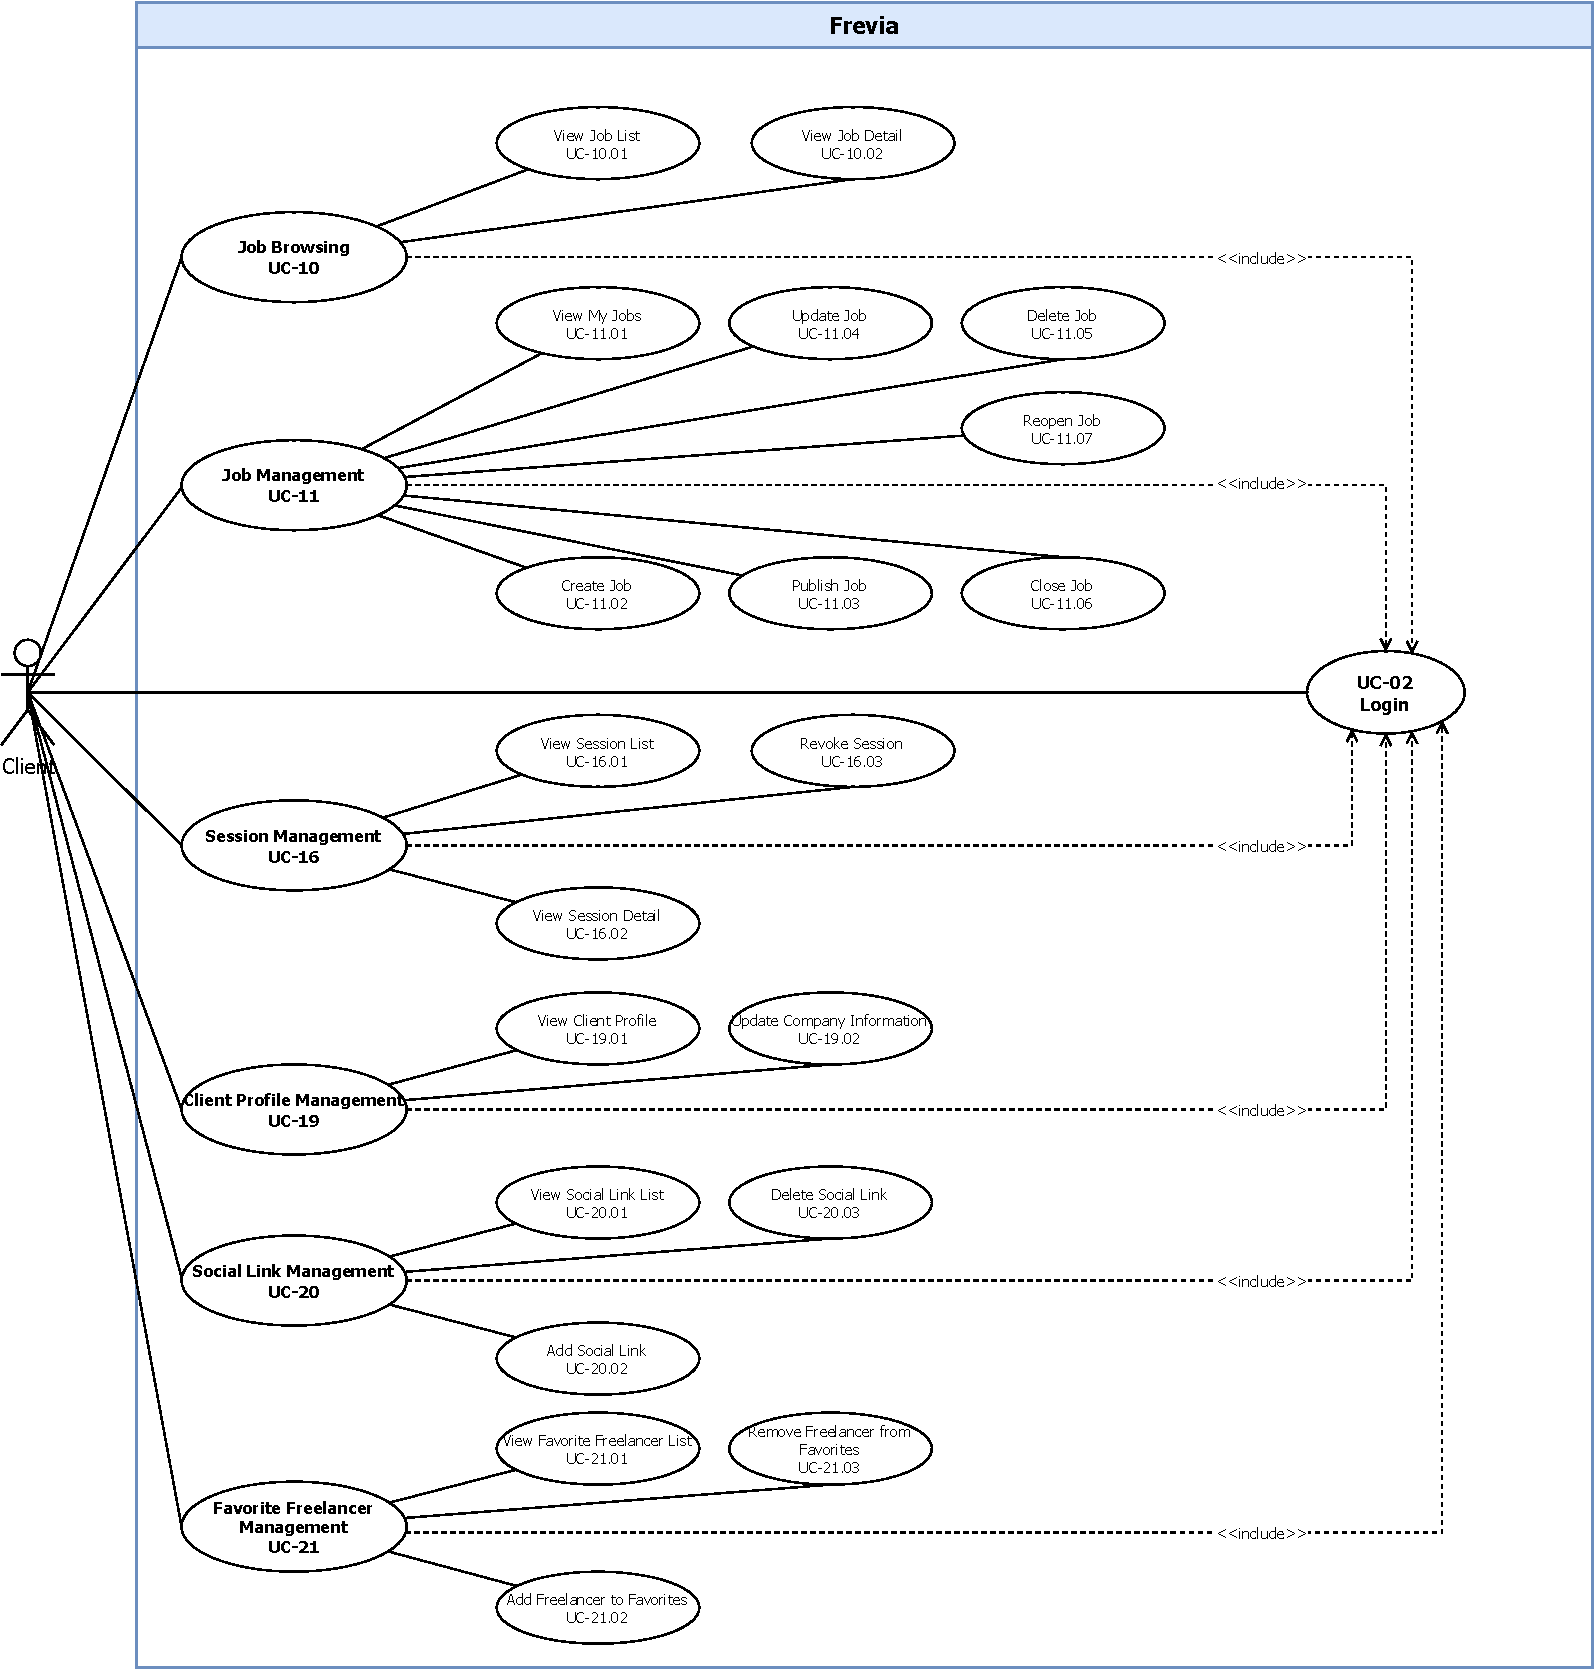
\includegraphics[
        width=\textwidth,
        height=0.85\textheight,
        keepaspectratio
    ]{image/UC_diagram/Client_2.pdf}
    \caption{Client Usecase 2/6}
    \label{fig:uc_client_2}
\end{figure}

\begin{figure}[H]
    \centering
    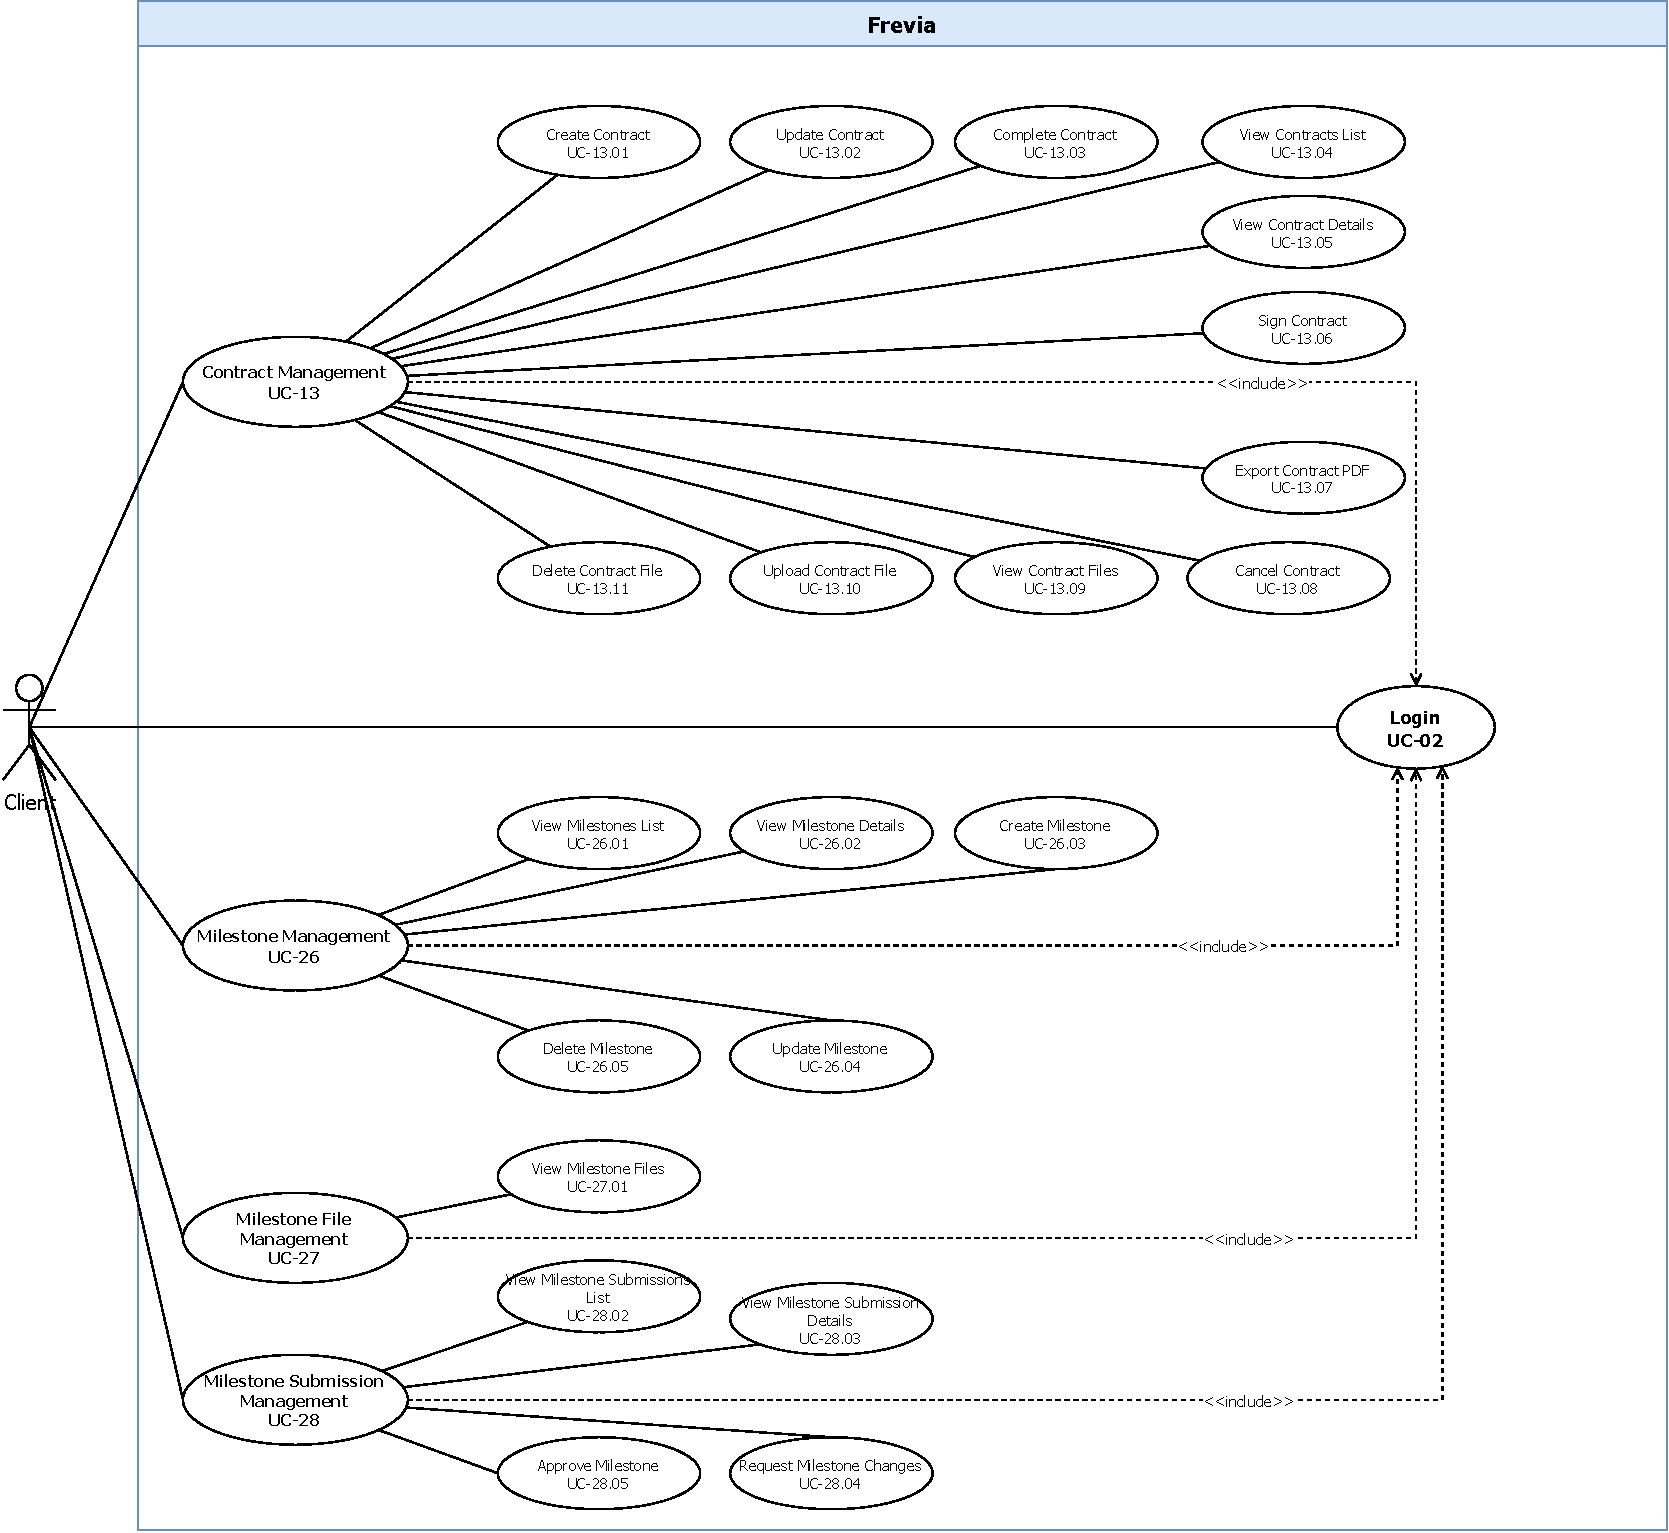
\includegraphics[
        width=\textwidth,
        height=0.85\textheight,
        keepaspectratio
    ]{image/UC_diagram/Client_3.pdf}
    \caption{Client Usecase 3/6}
    \label{fig:uc_client_3}
\end{figure}

\begin{figure}[H]
    \centering
    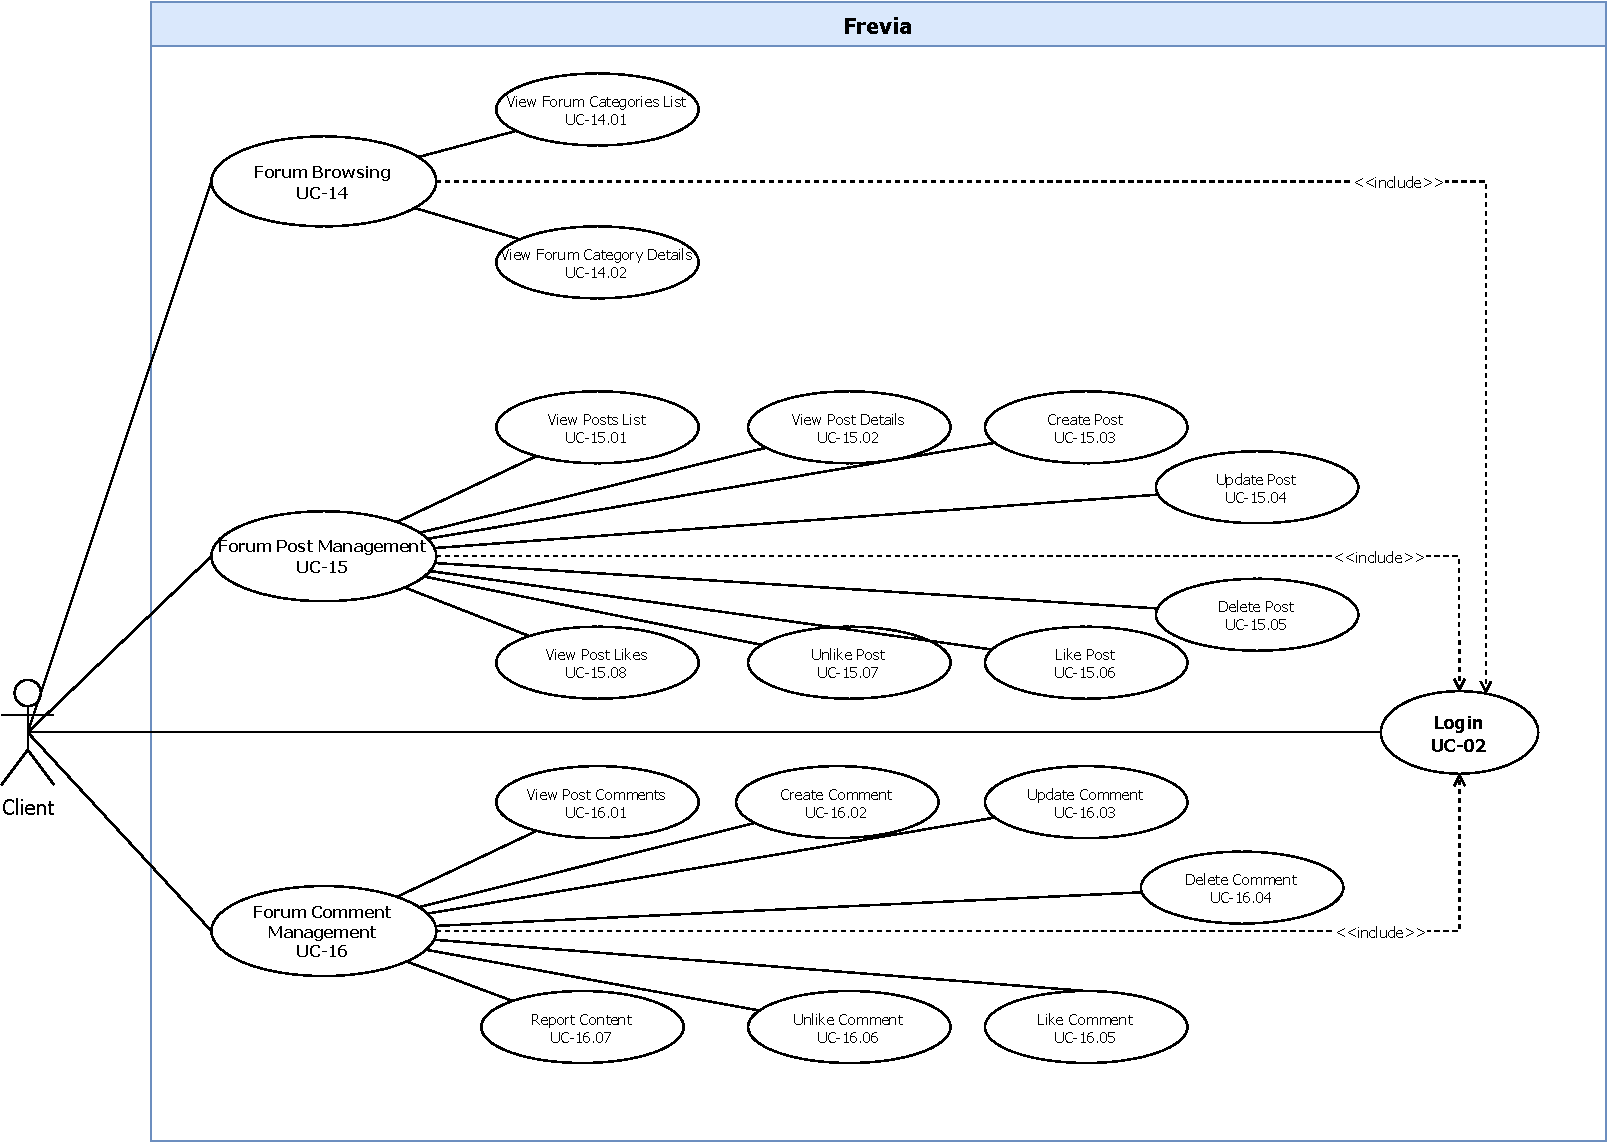
\includegraphics[
        width=\textwidth,
        height=0.85\textheight,
        keepaspectratio
    ]{image/UC_diagram/Client_4.pdf}
    \caption{Client Usecase 4/6}
    \label{fig:uc_client_4}
\end{figure}

\begin{figure}[H]
    \centering
    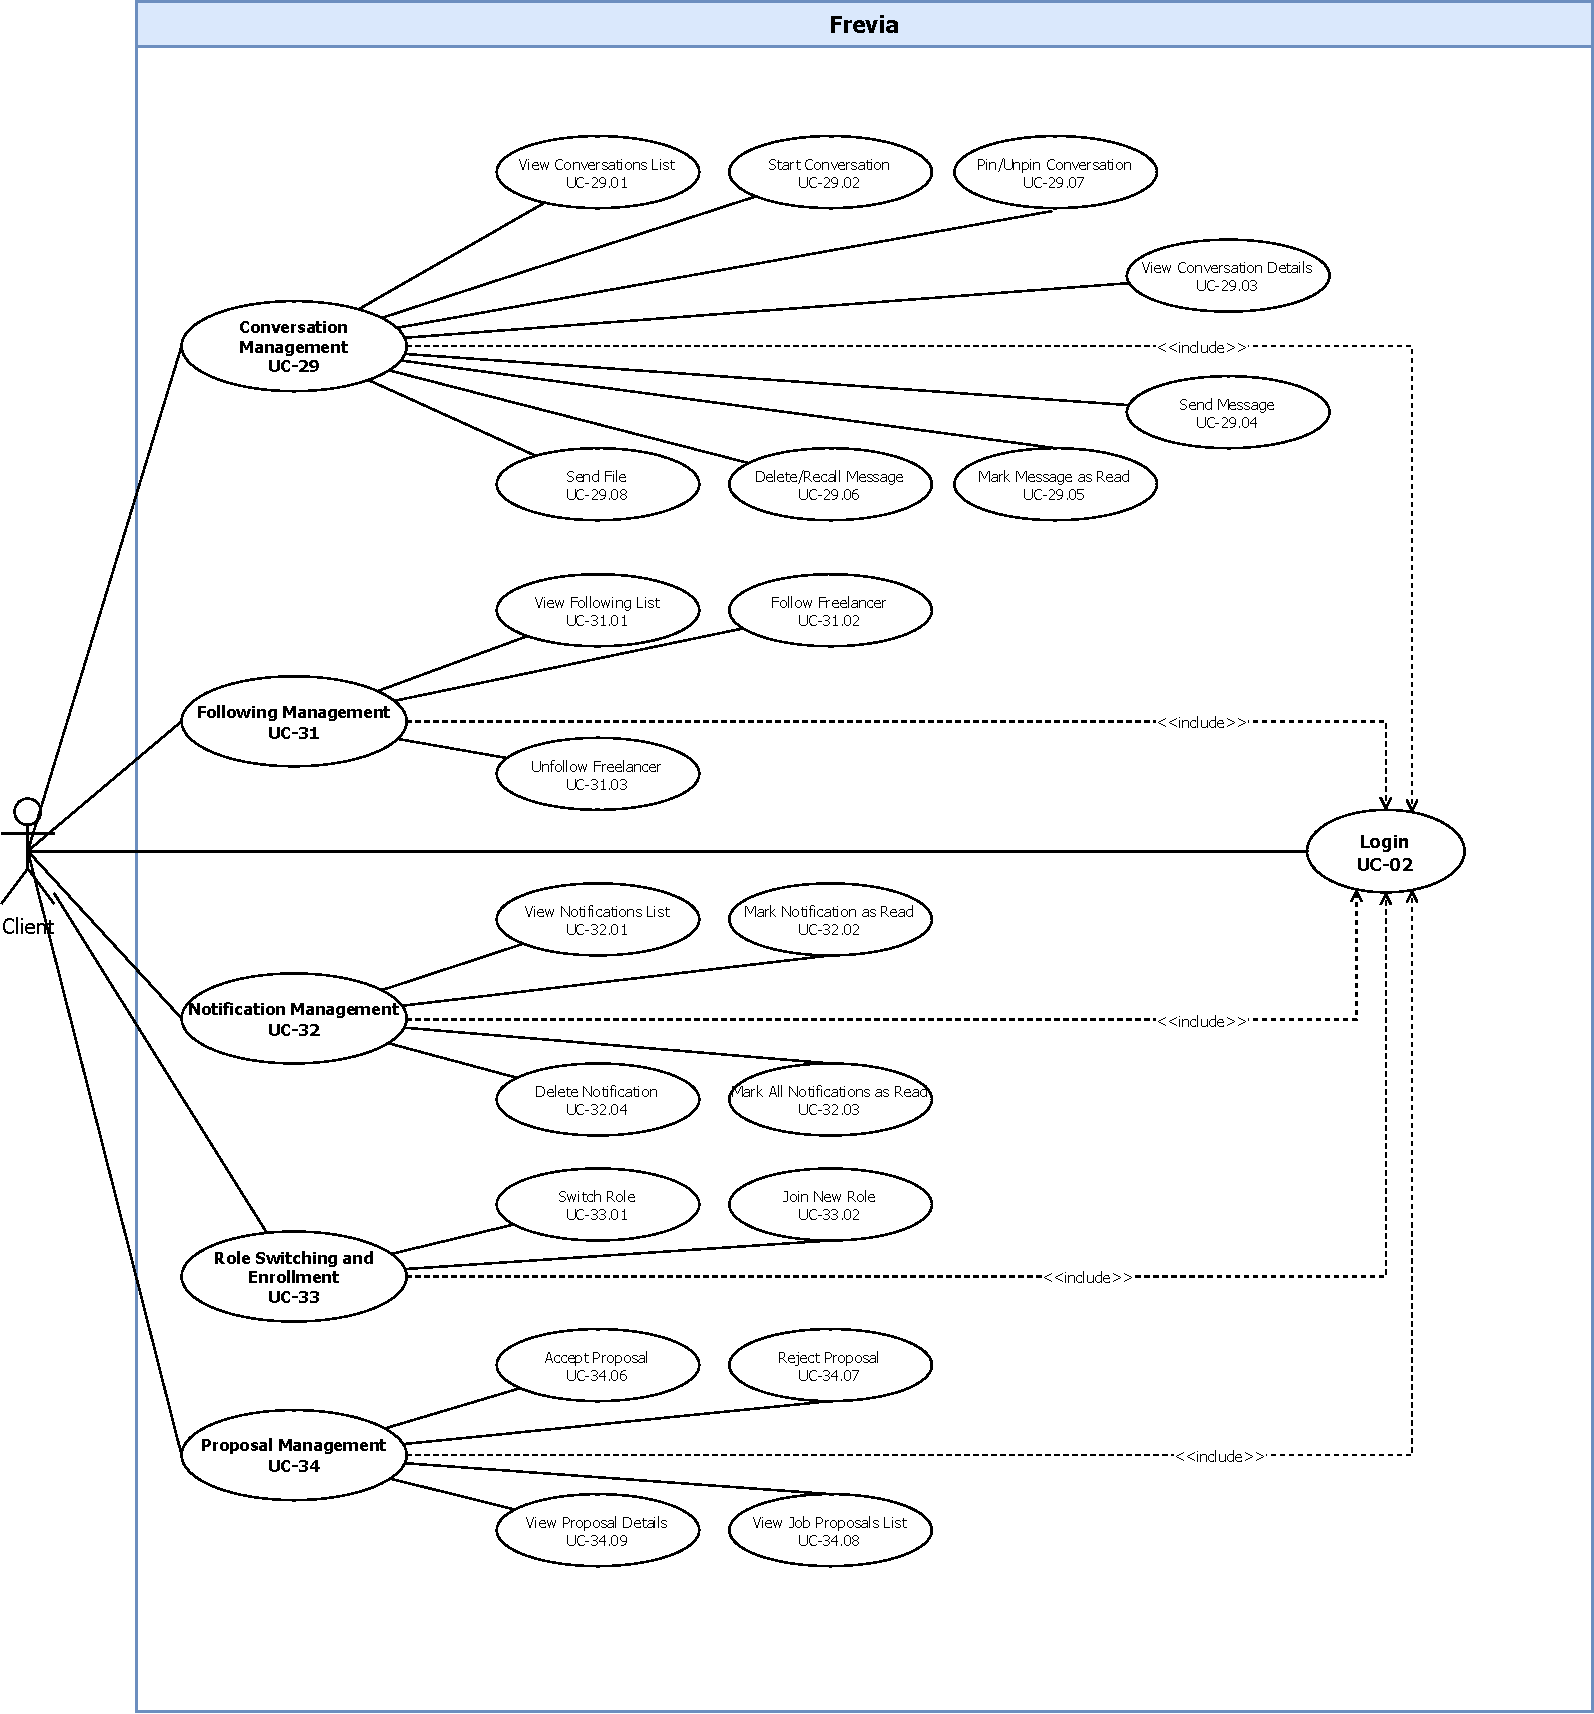
\includegraphics[
        width=\textwidth,
        height=0.85\textheight,
        keepaspectratio
    ]{image/UC_diagram/Client_5.pdf}
    \caption{Client Usecase 5/6}
    \label{fig:uc_client_5}
\end{figure}

\begin{figure}[H]
    \centering
    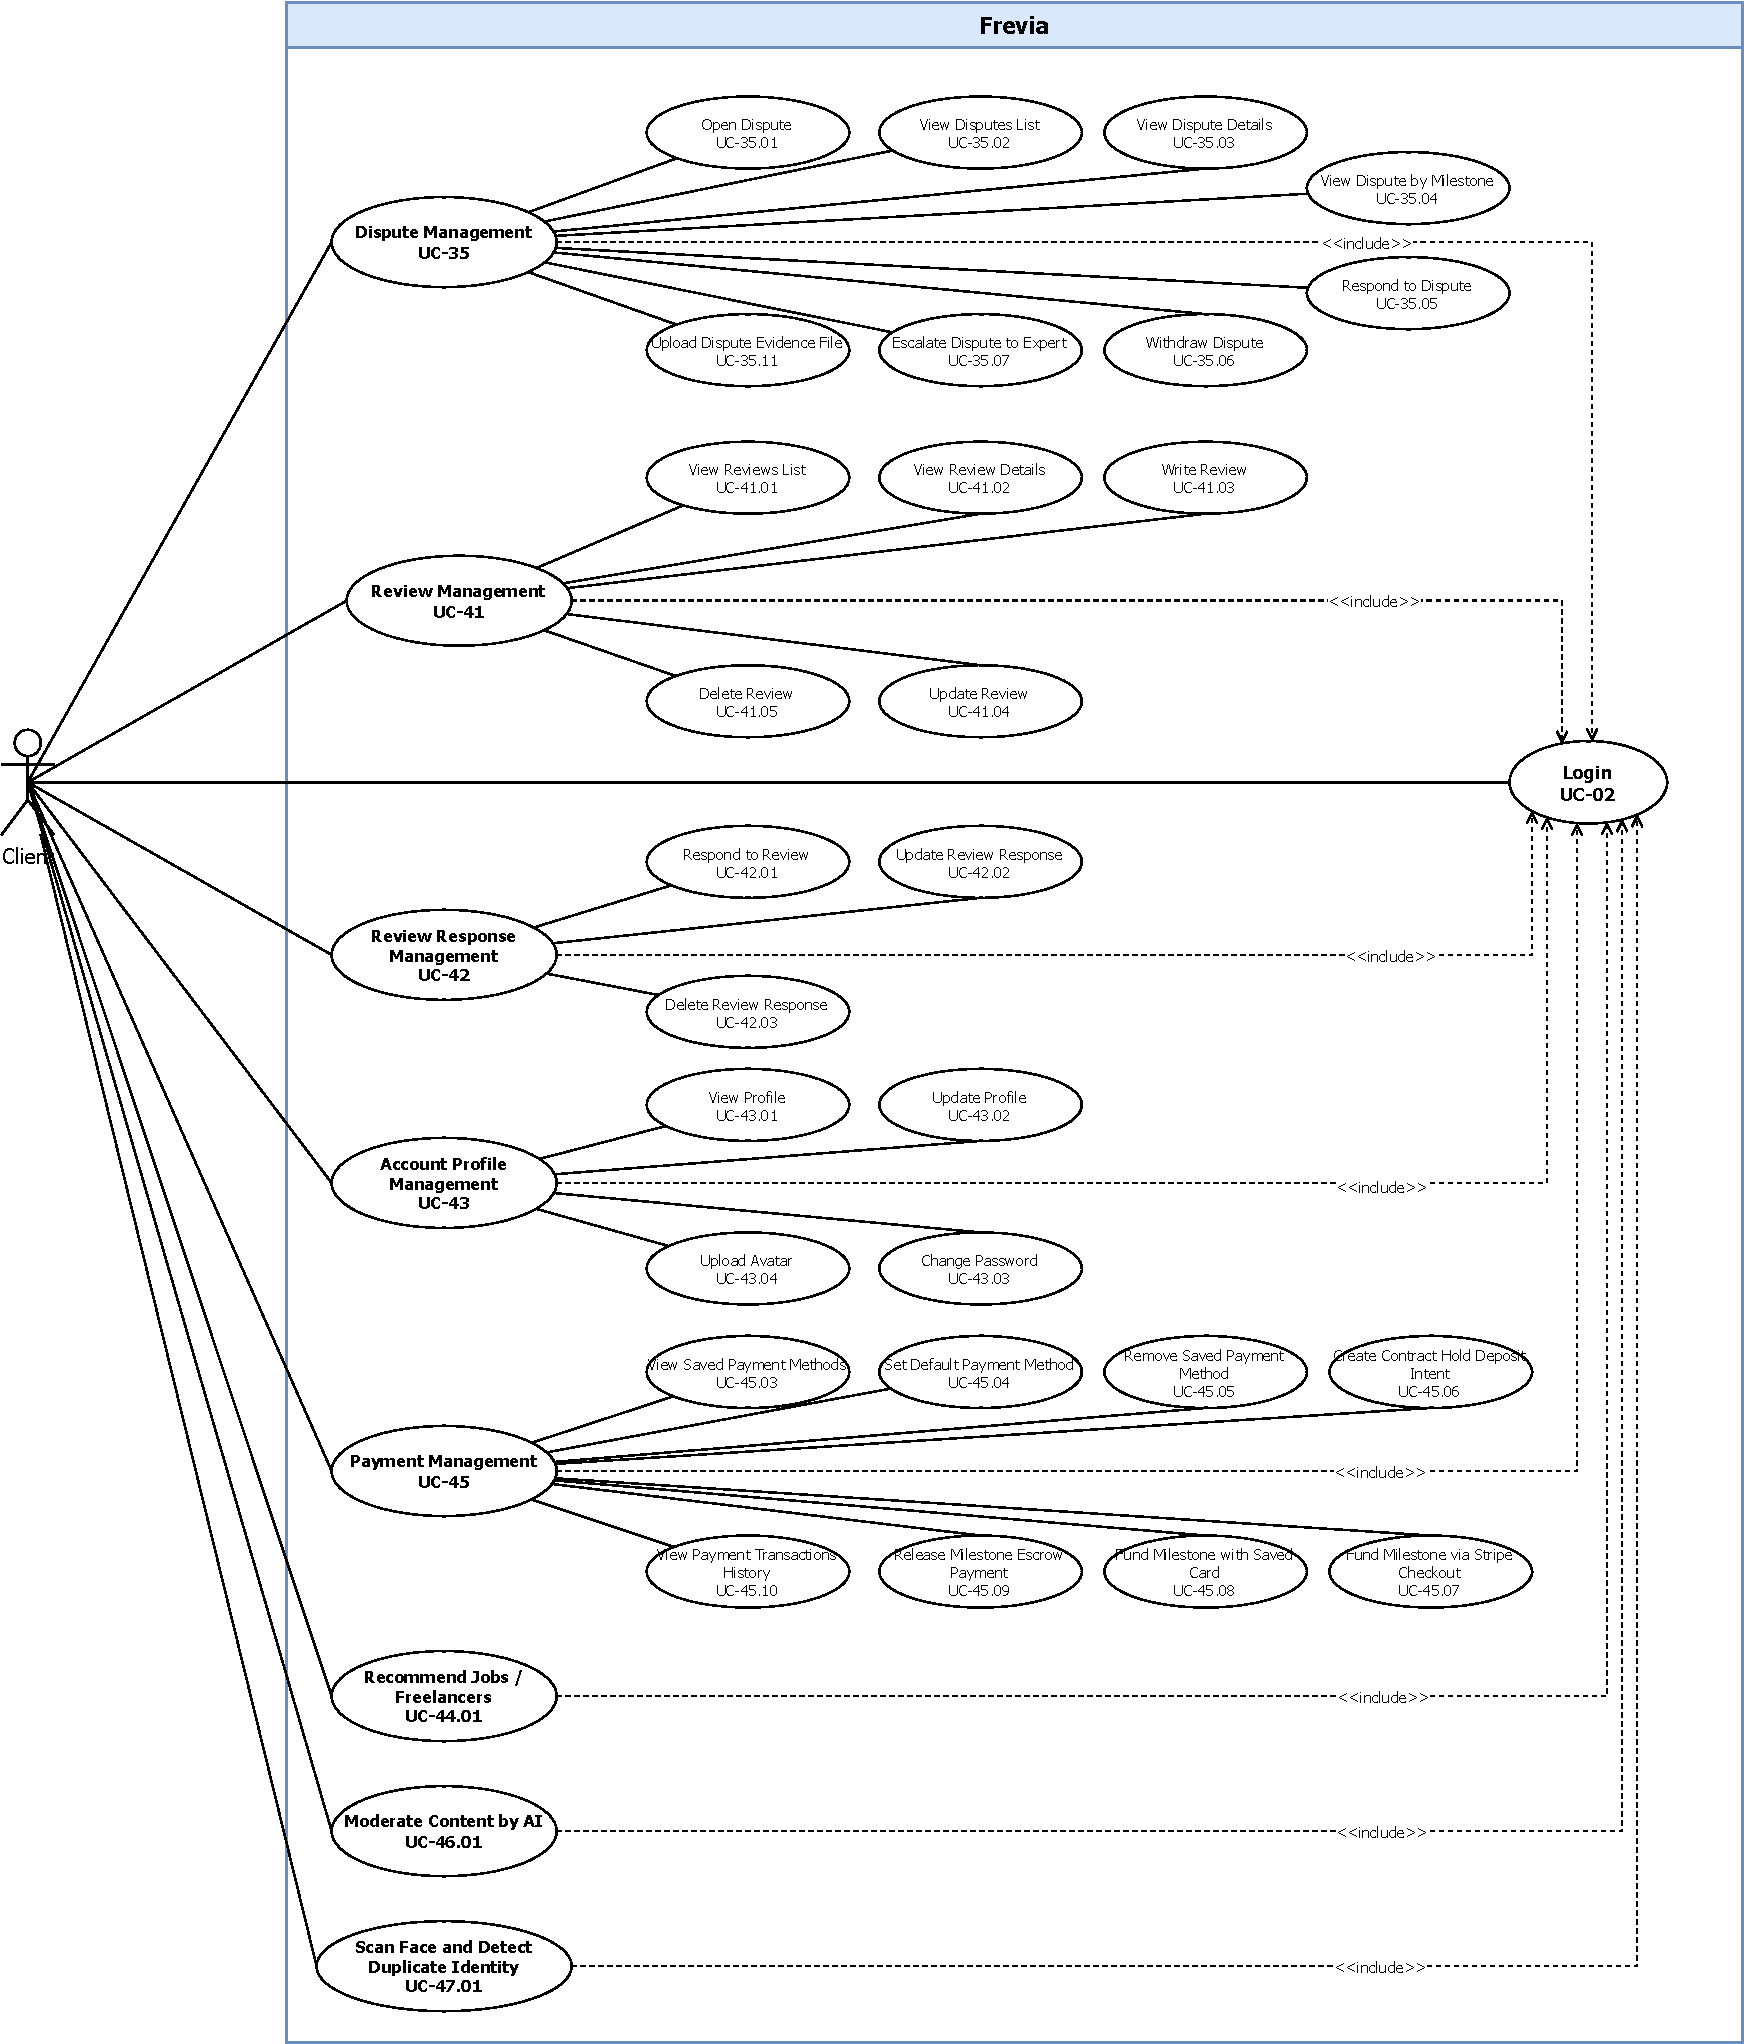
\includegraphics[
        width=\textwidth,
        height=0.85\textheight,
        keepaspectratio
    ]{image/UC_diagram/Client_6.pdf}
    \caption{Client Usecase 6/6}
    \label{fig:uc_client_6}
\end{figure}

% =========================================================================
% 3. Freelancer Use Case Diagrams
% =========================================================================
\begin{figure}[H]
    \centering
    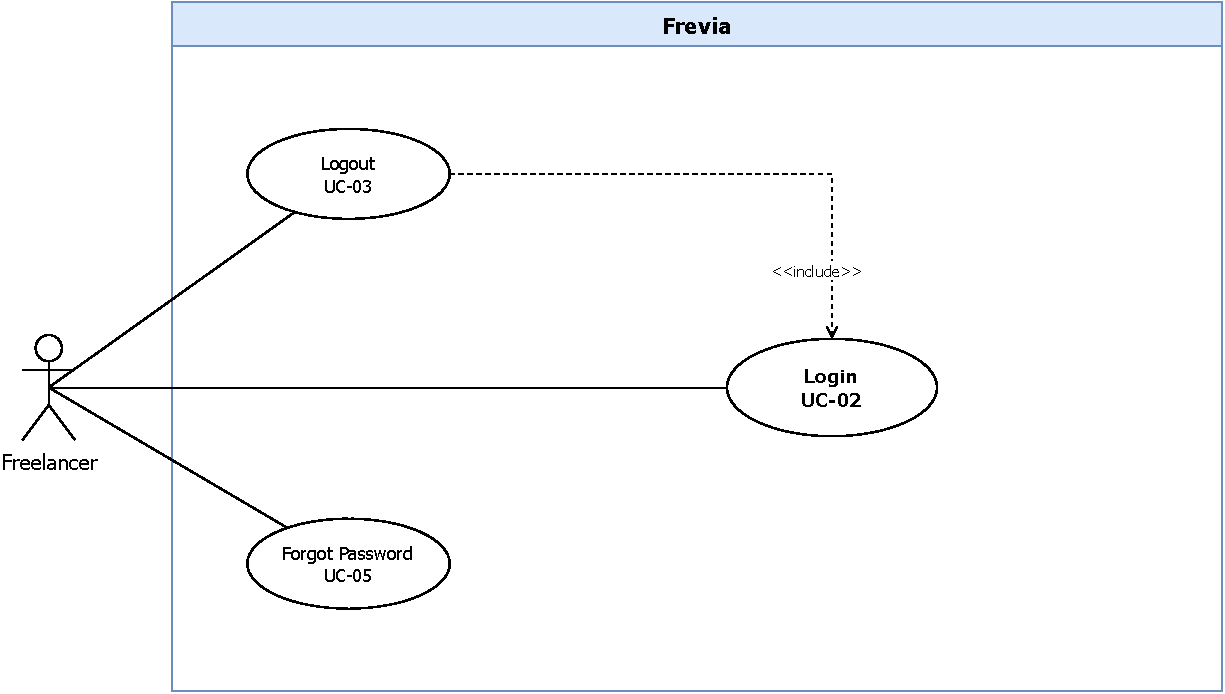
\includegraphics[
        width=\textwidth,
        height=0.85\textheight,
        keepaspectratio
    ]{image/UC_diagram/Freelancer_1.pdf}
    \caption{Freelancer Usecase 1/7}
    \label{fig:uc_freelancer_1}
\end{figure}

\begin{figure}[H]
    \centering
    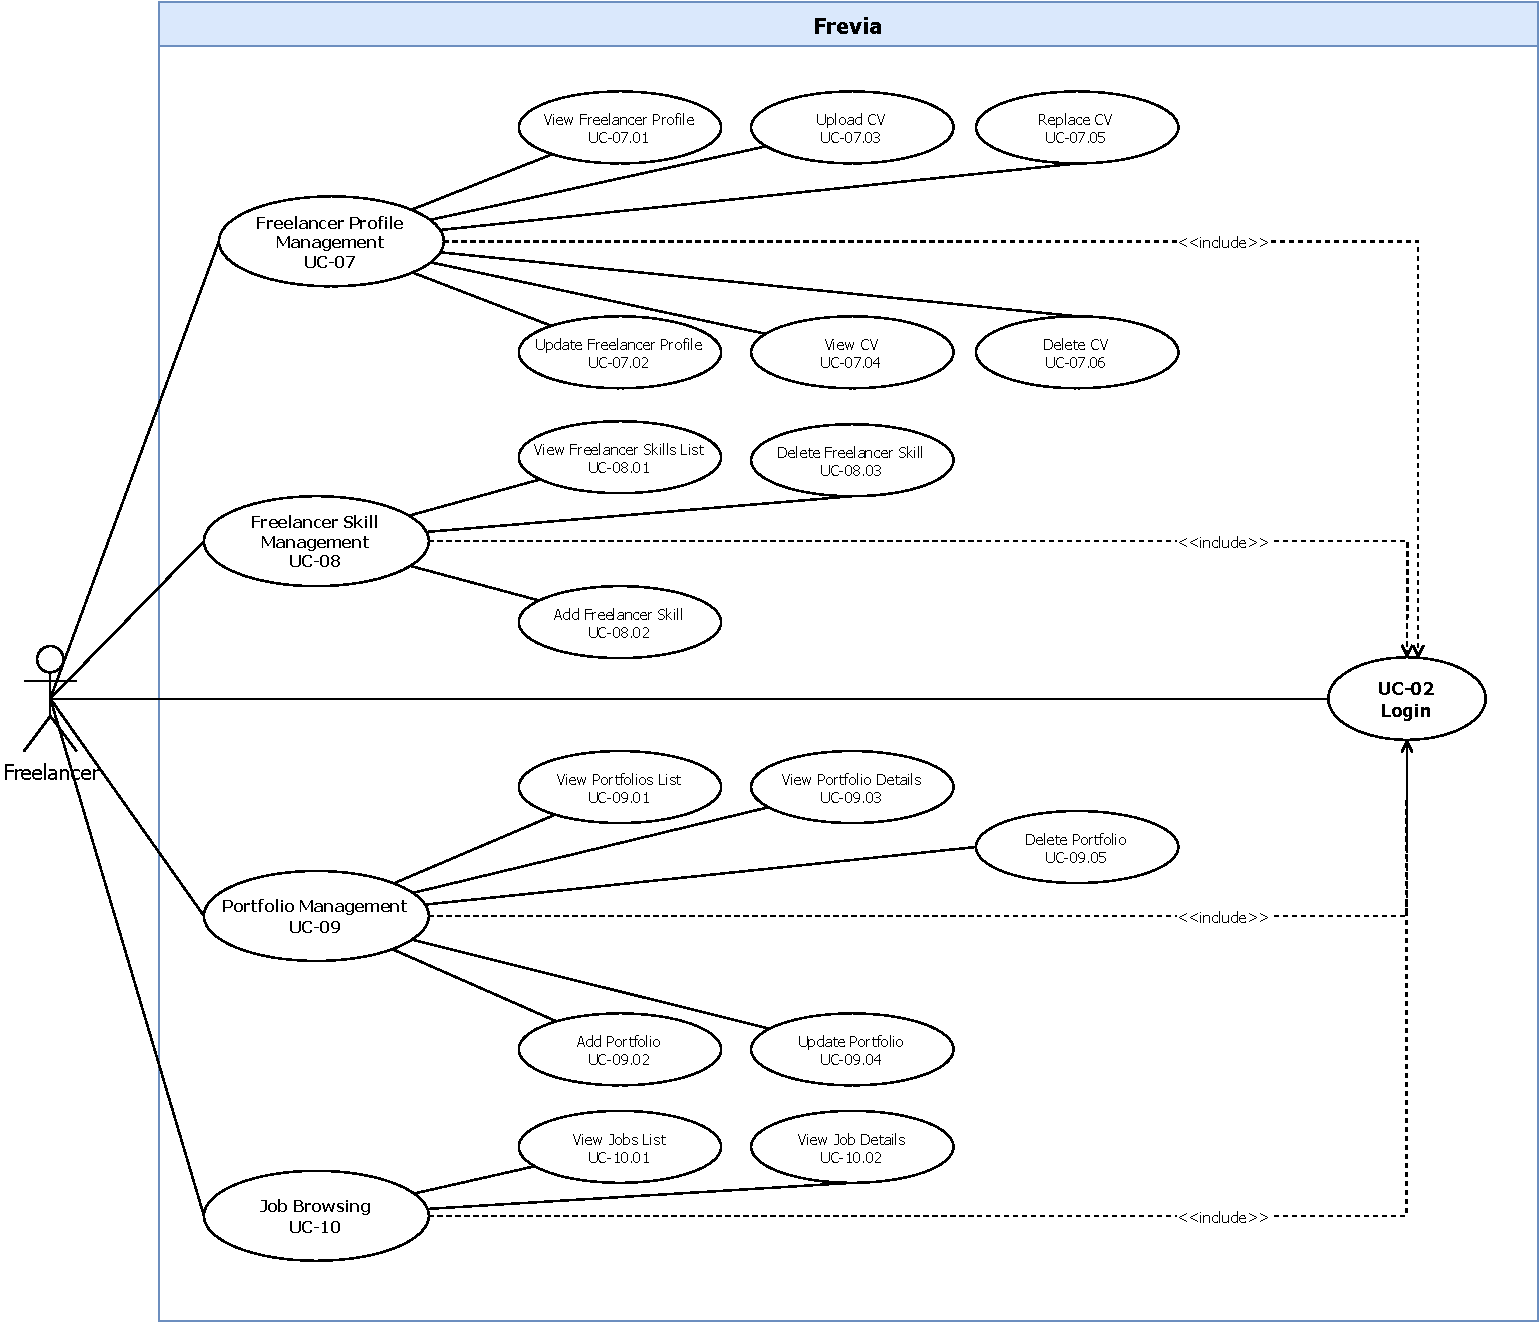
\includegraphics[
        width=\textwidth,
        height=0.85\textheight,
        keepaspectratio
    ]{image/UC_diagram/Freelancer_2.pdf}
    \caption{Freelancer Usecase 2/7}
    \label{fig:uc_freelancer_2}
\end{figure}

\begin{figure}[H]
    \centering
    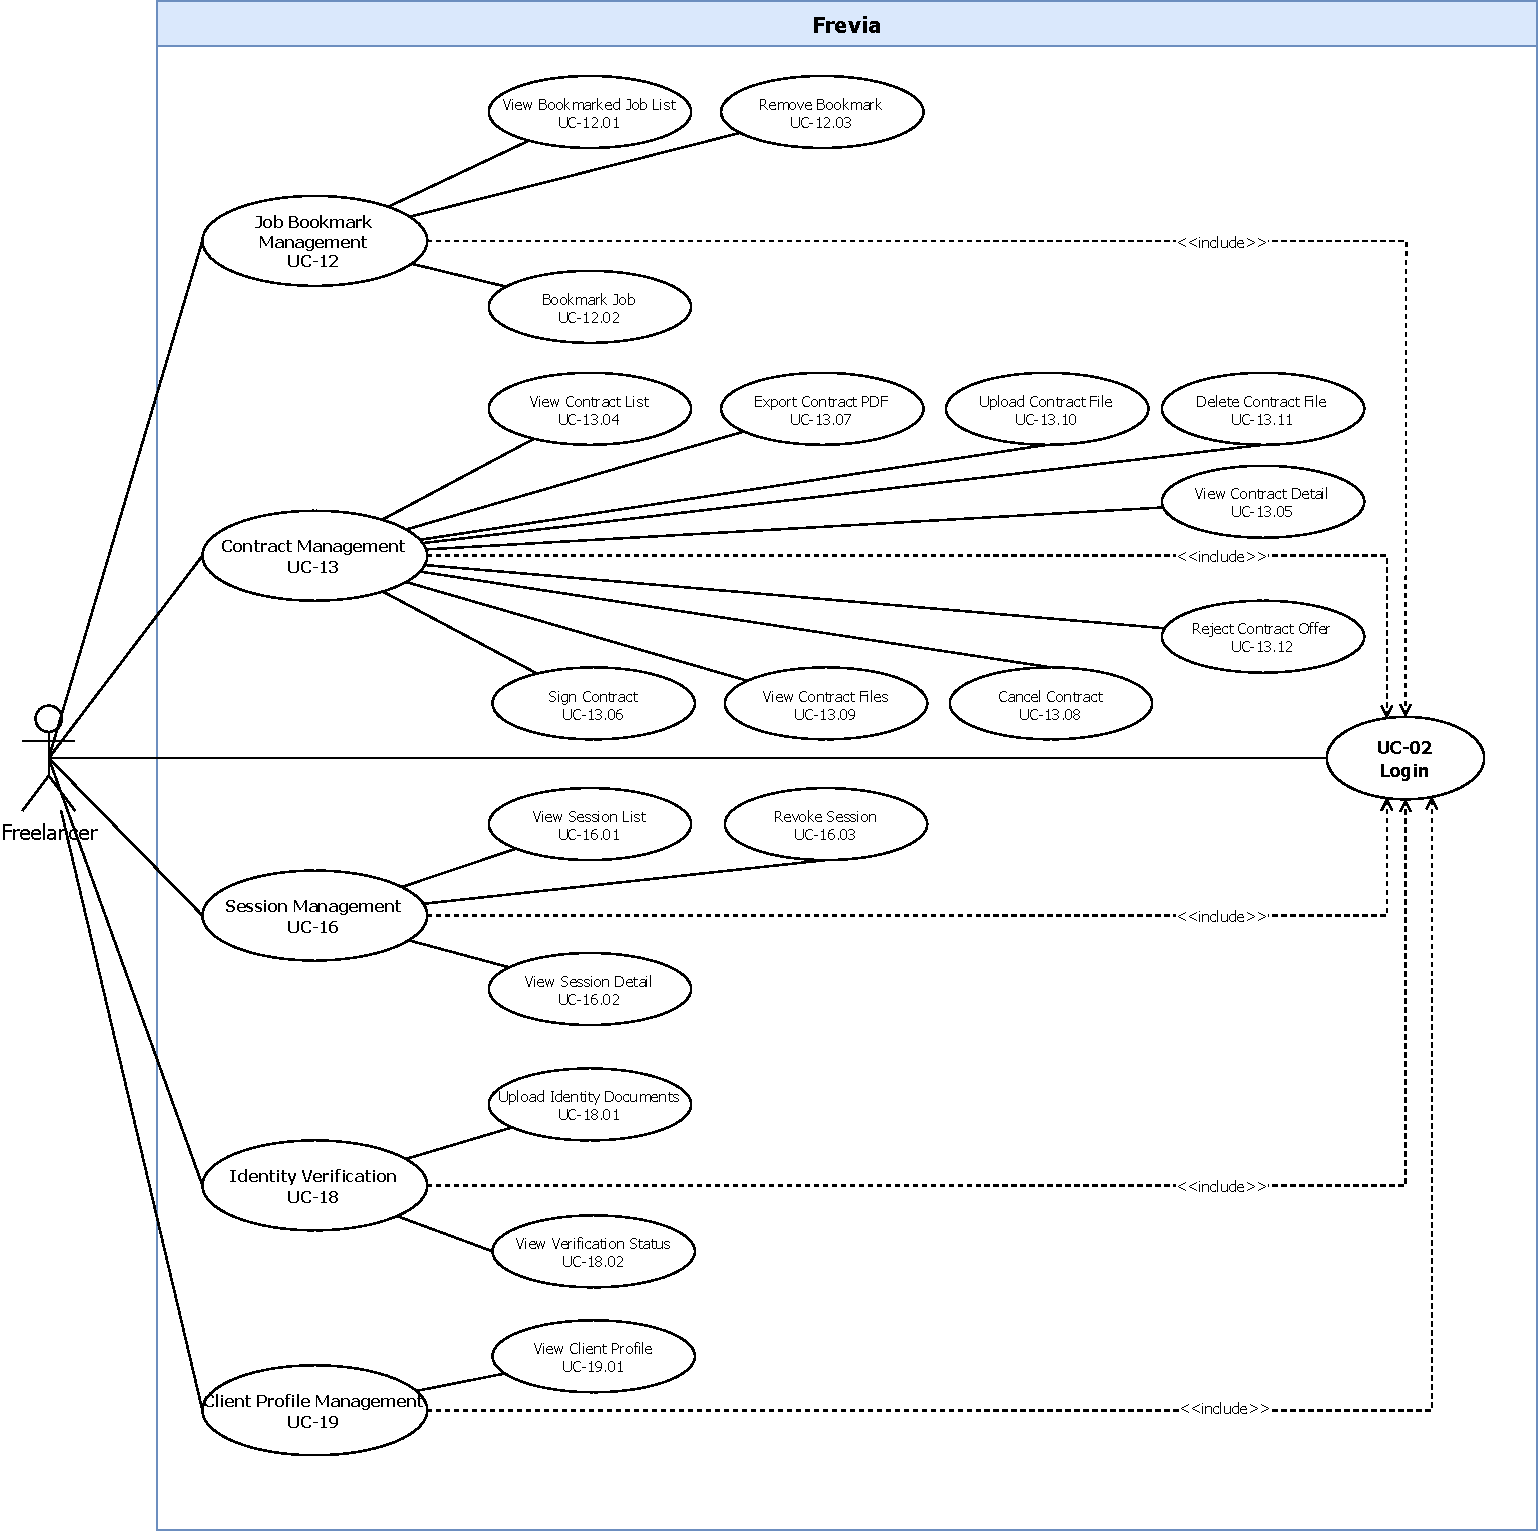
\includegraphics[
        width=\textwidth,
        height=0.85\textheight,
        keepaspectratio
    ]{image/UC_diagram/Freelancer_3.pdf}
    \caption{Freelancer Usecase 3/7}
    \label{fig:uc_freelancer_3}
\end{figure}

\begin{figure}[H]
    \centering
    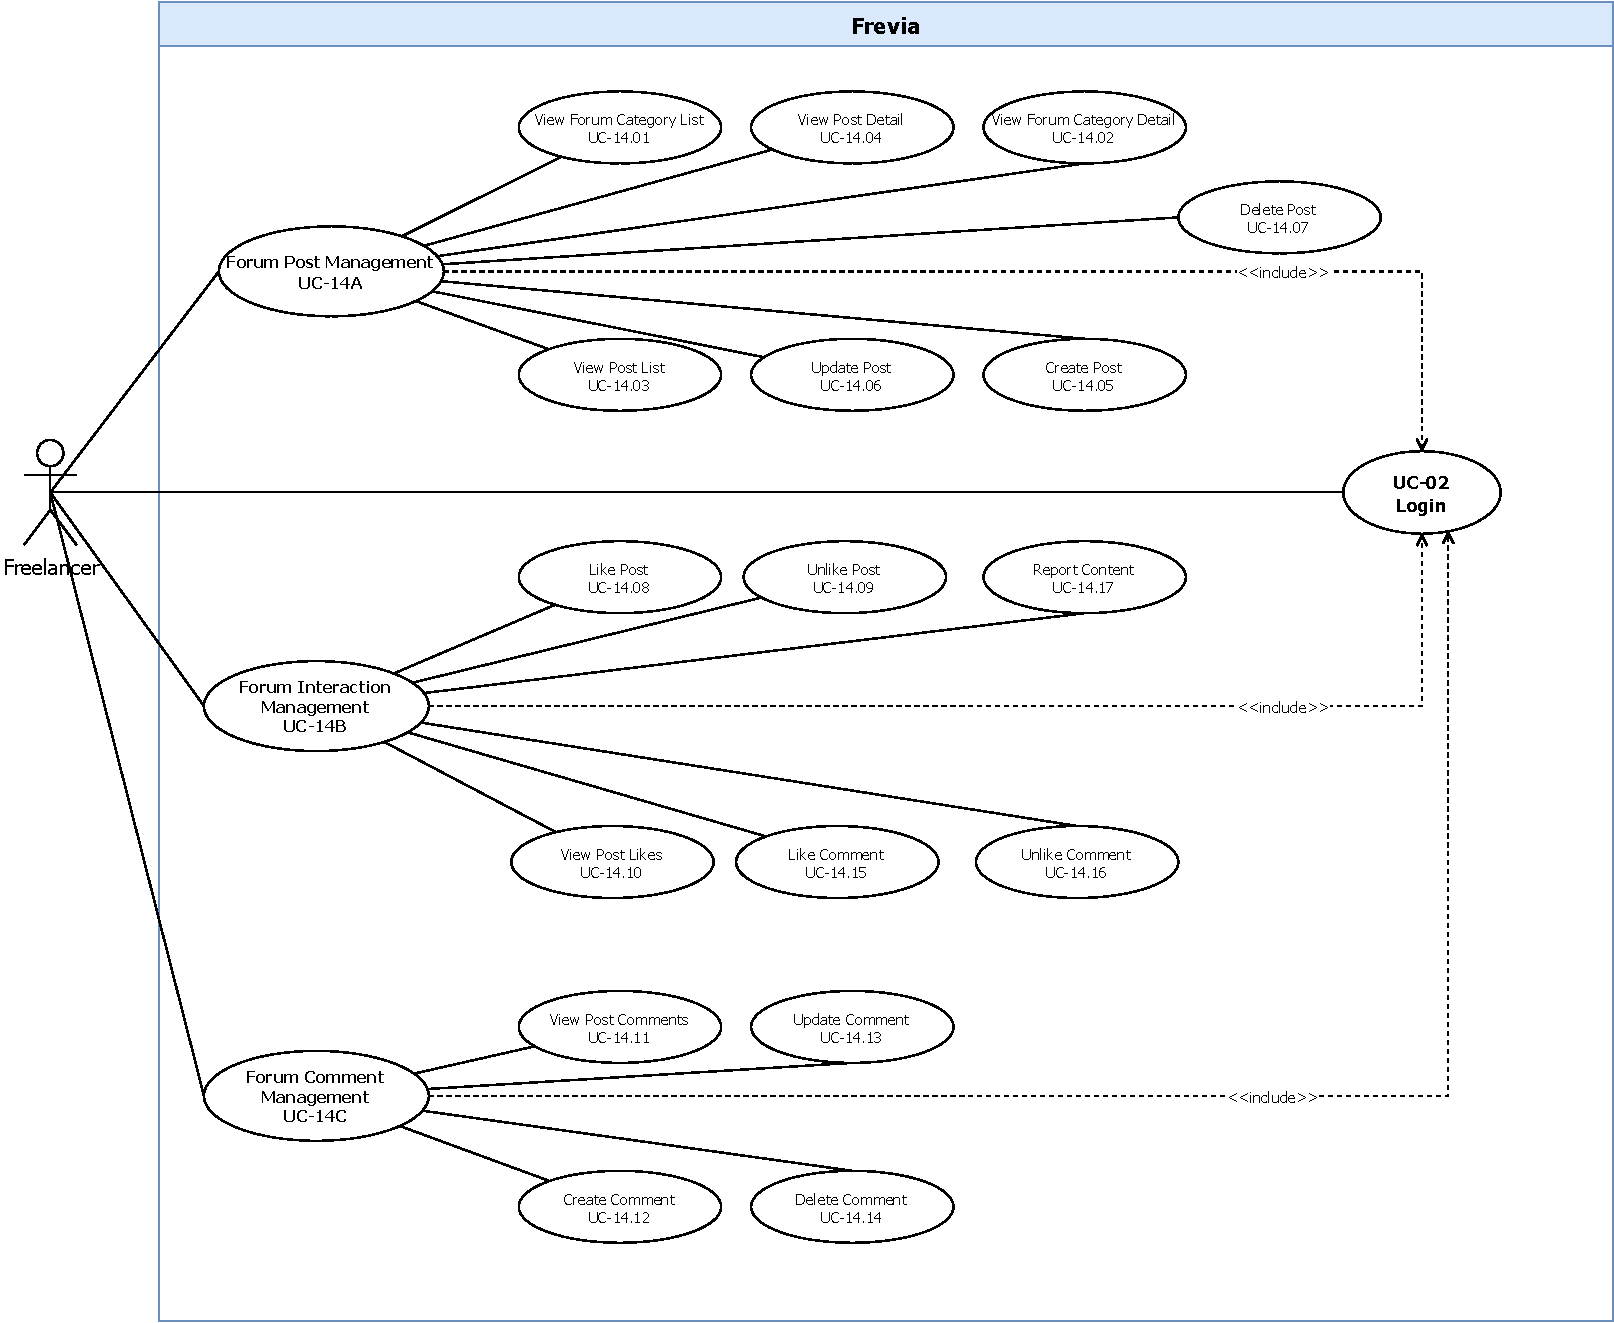
\includegraphics[
        width=\textwidth,
        height=0.85\textheight,
        keepaspectratio
    ]{image/UC_diagram/Freelancer_4.pdf}
    \caption{Freelancer Usecase 4/7}
    \label{fig:uc_freelancer_4}
\end{figure}

\begin{figure}[H]
    \centering
    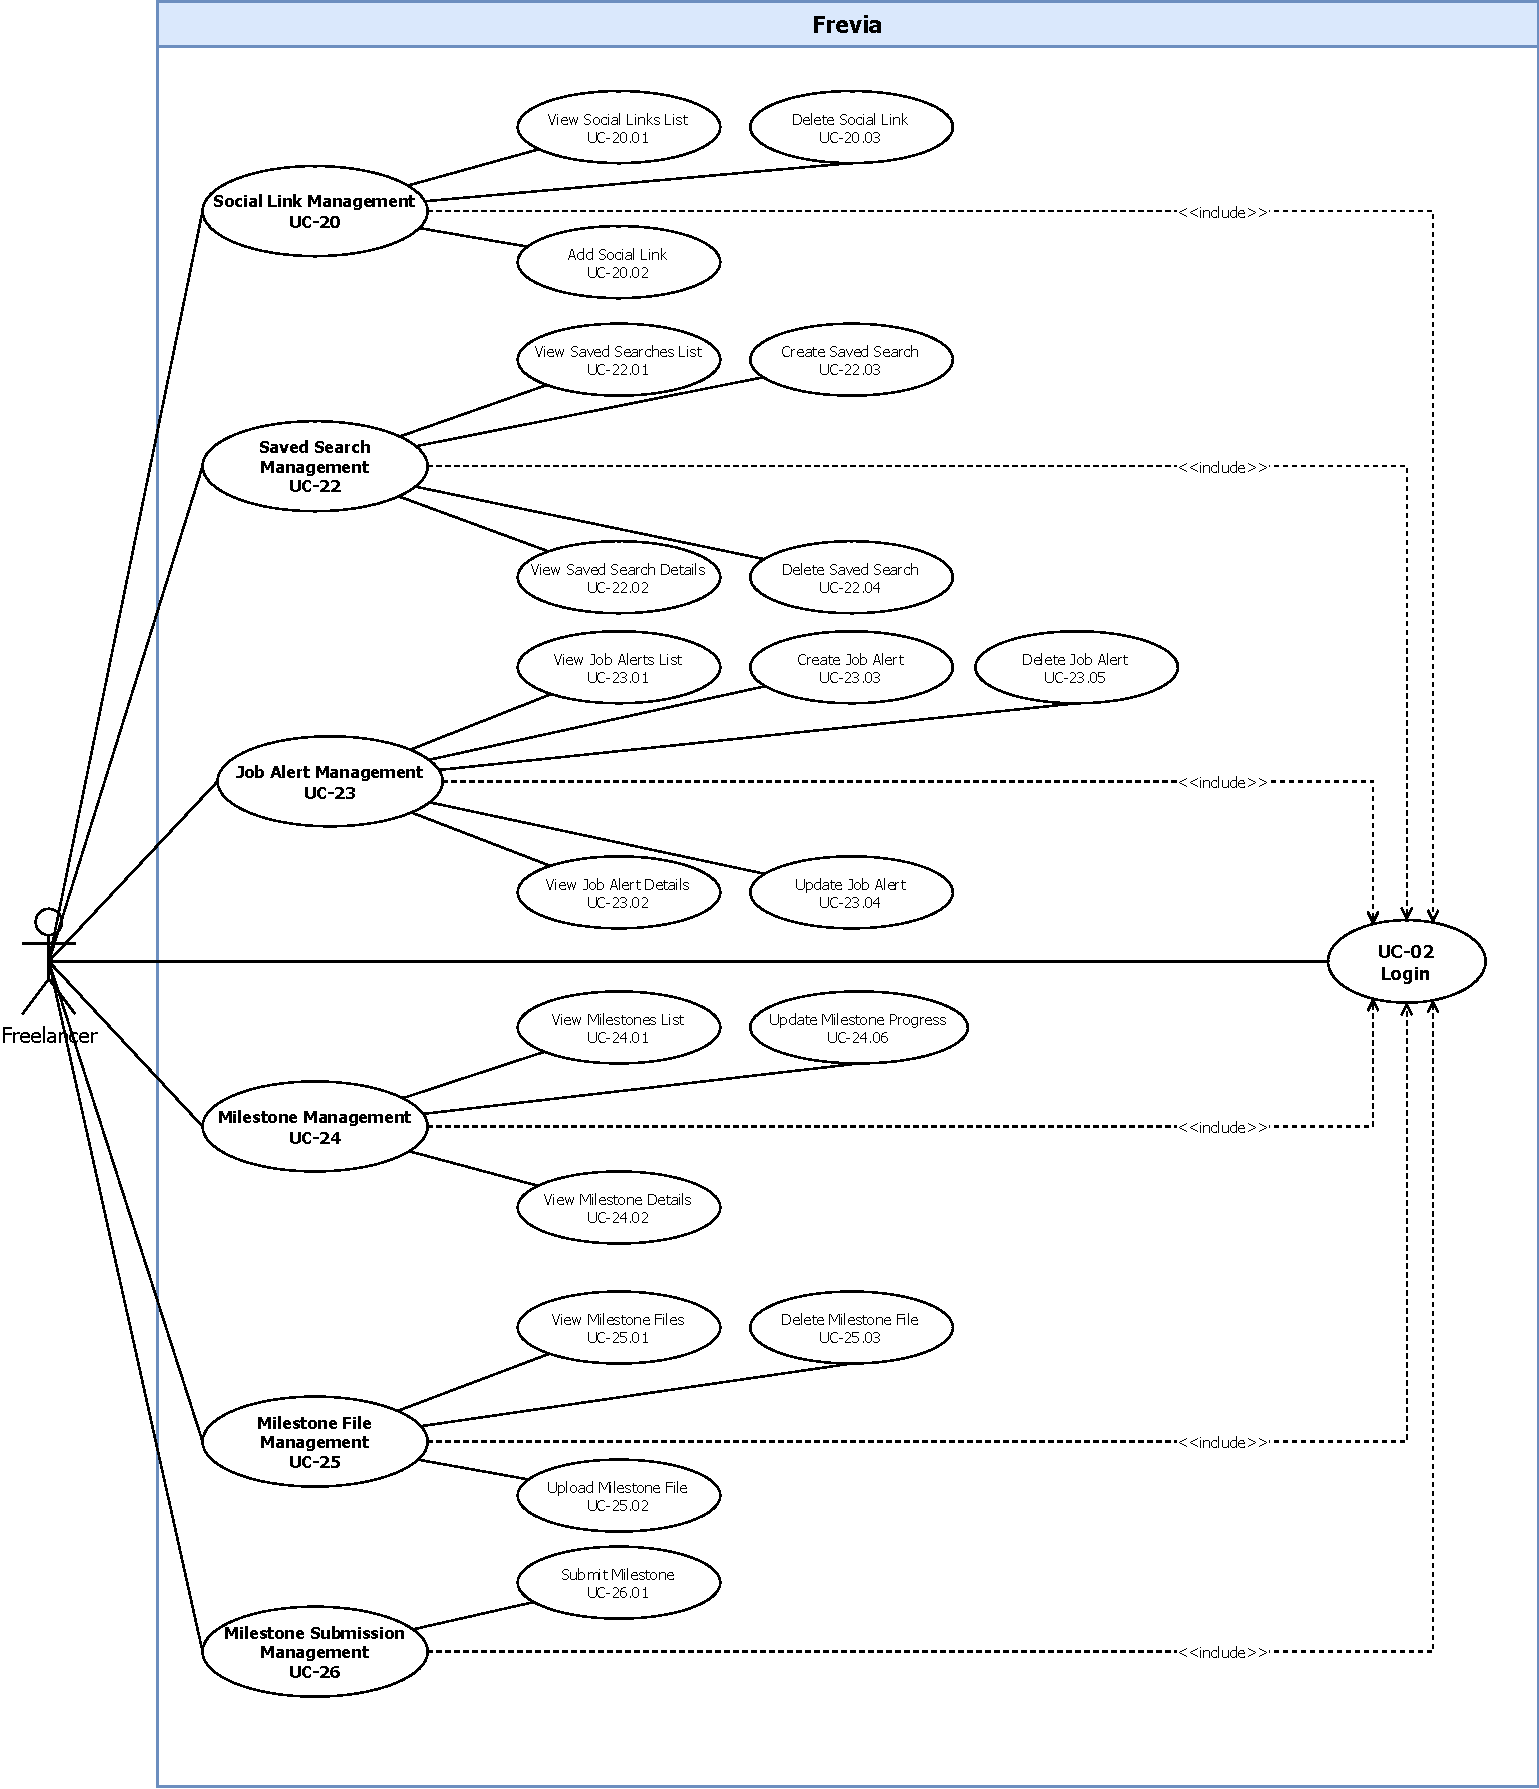
\includegraphics[
        width=\textwidth,
        height=0.85\textheight,
        keepaspectratio
    ]{image/UC_diagram/Freelancer_5.pdf}
    \caption{Freelancer Usecase 5/7}
    \label{fig:uc_freelancer_5}
\end{figure}

\begin{figure}[H]
    \centering
    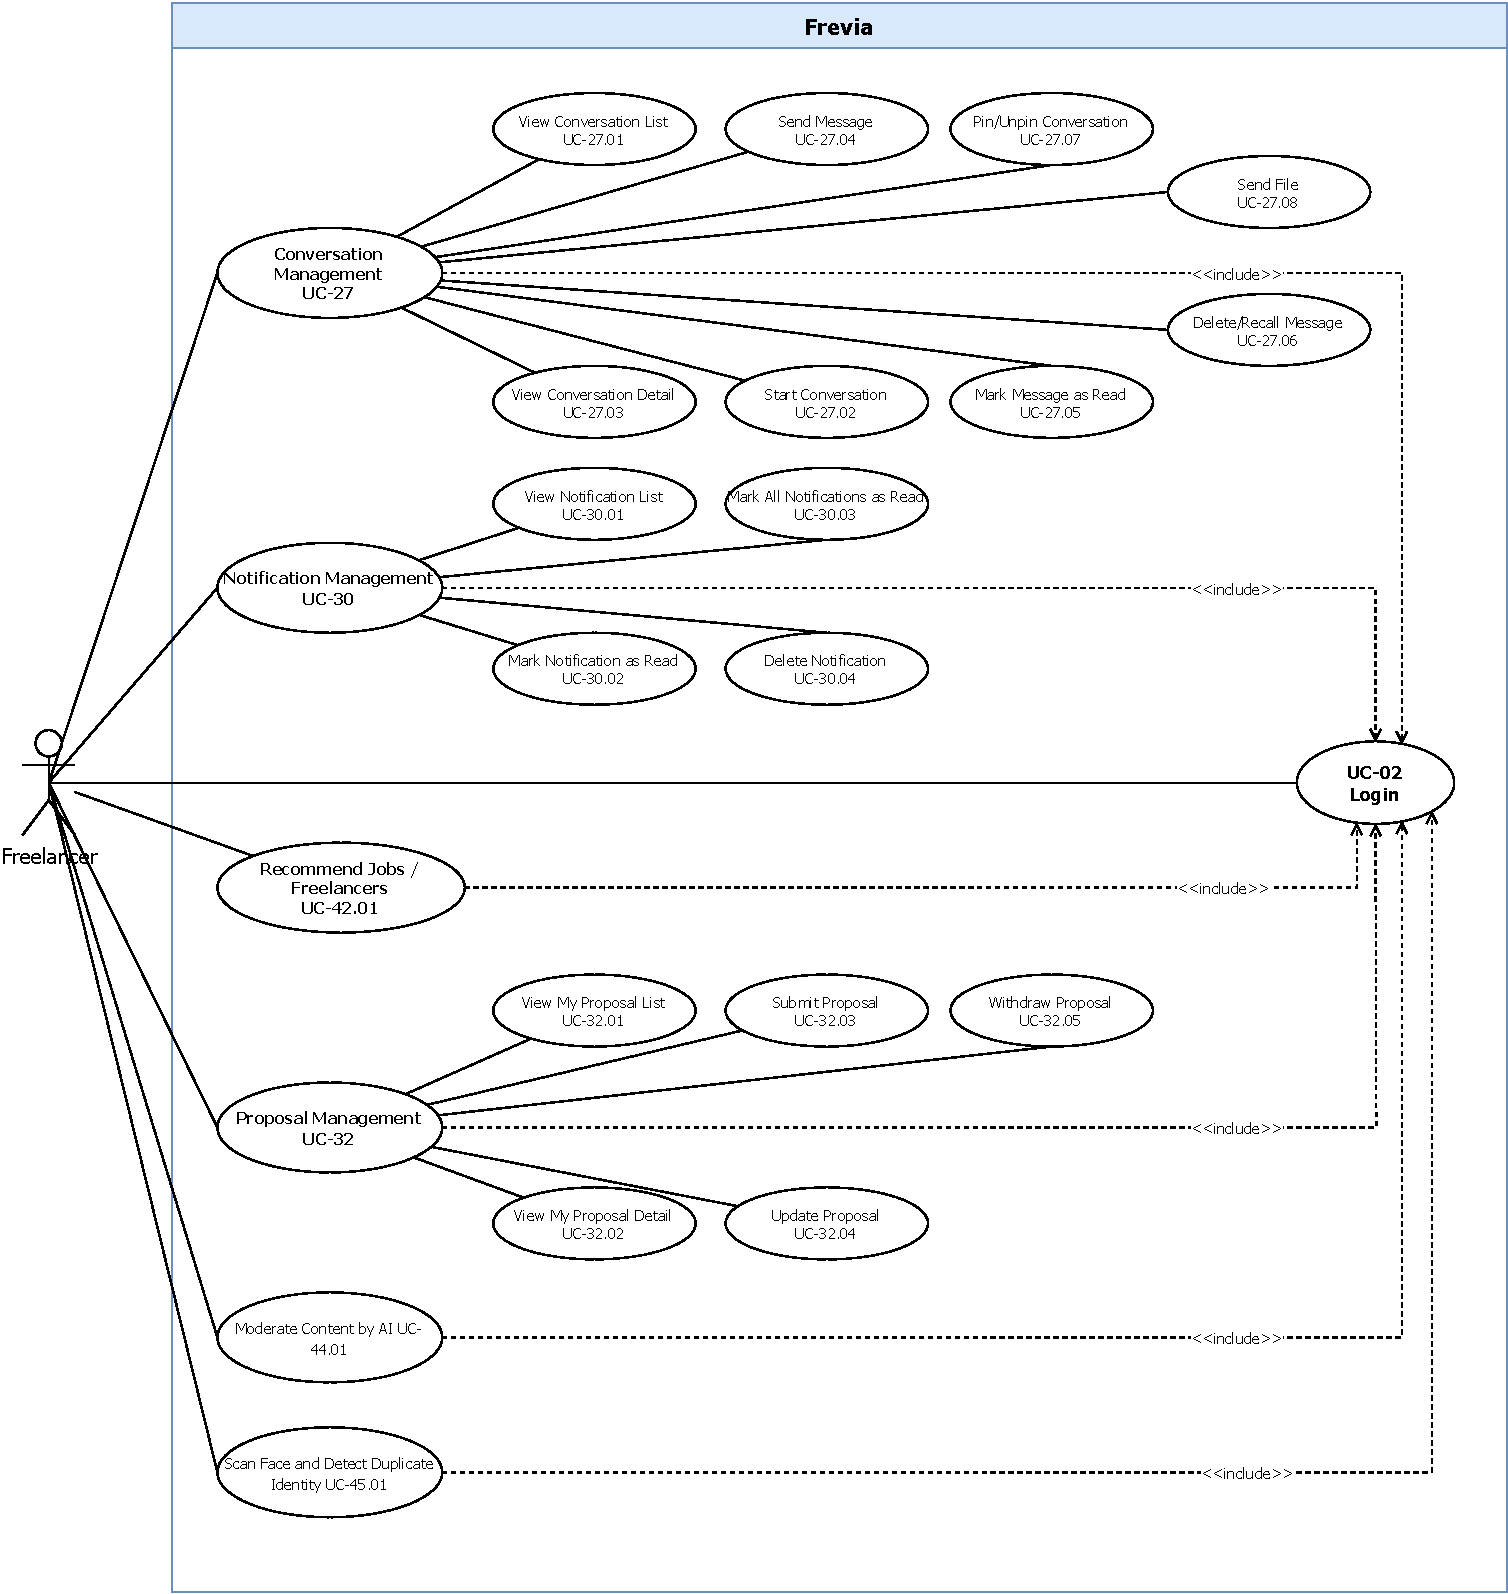
\includegraphics[
        width=\textwidth,
        height=0.85\textheight,
        keepaspectratio
    ]{image/UC_diagram/Freelancer_6.pdf}
    \caption{Freelancer Usecase 6/7}
    \label{fig:uc_freelancer_6}
\end{figure}

\begin{figure}[H]
    \centering
    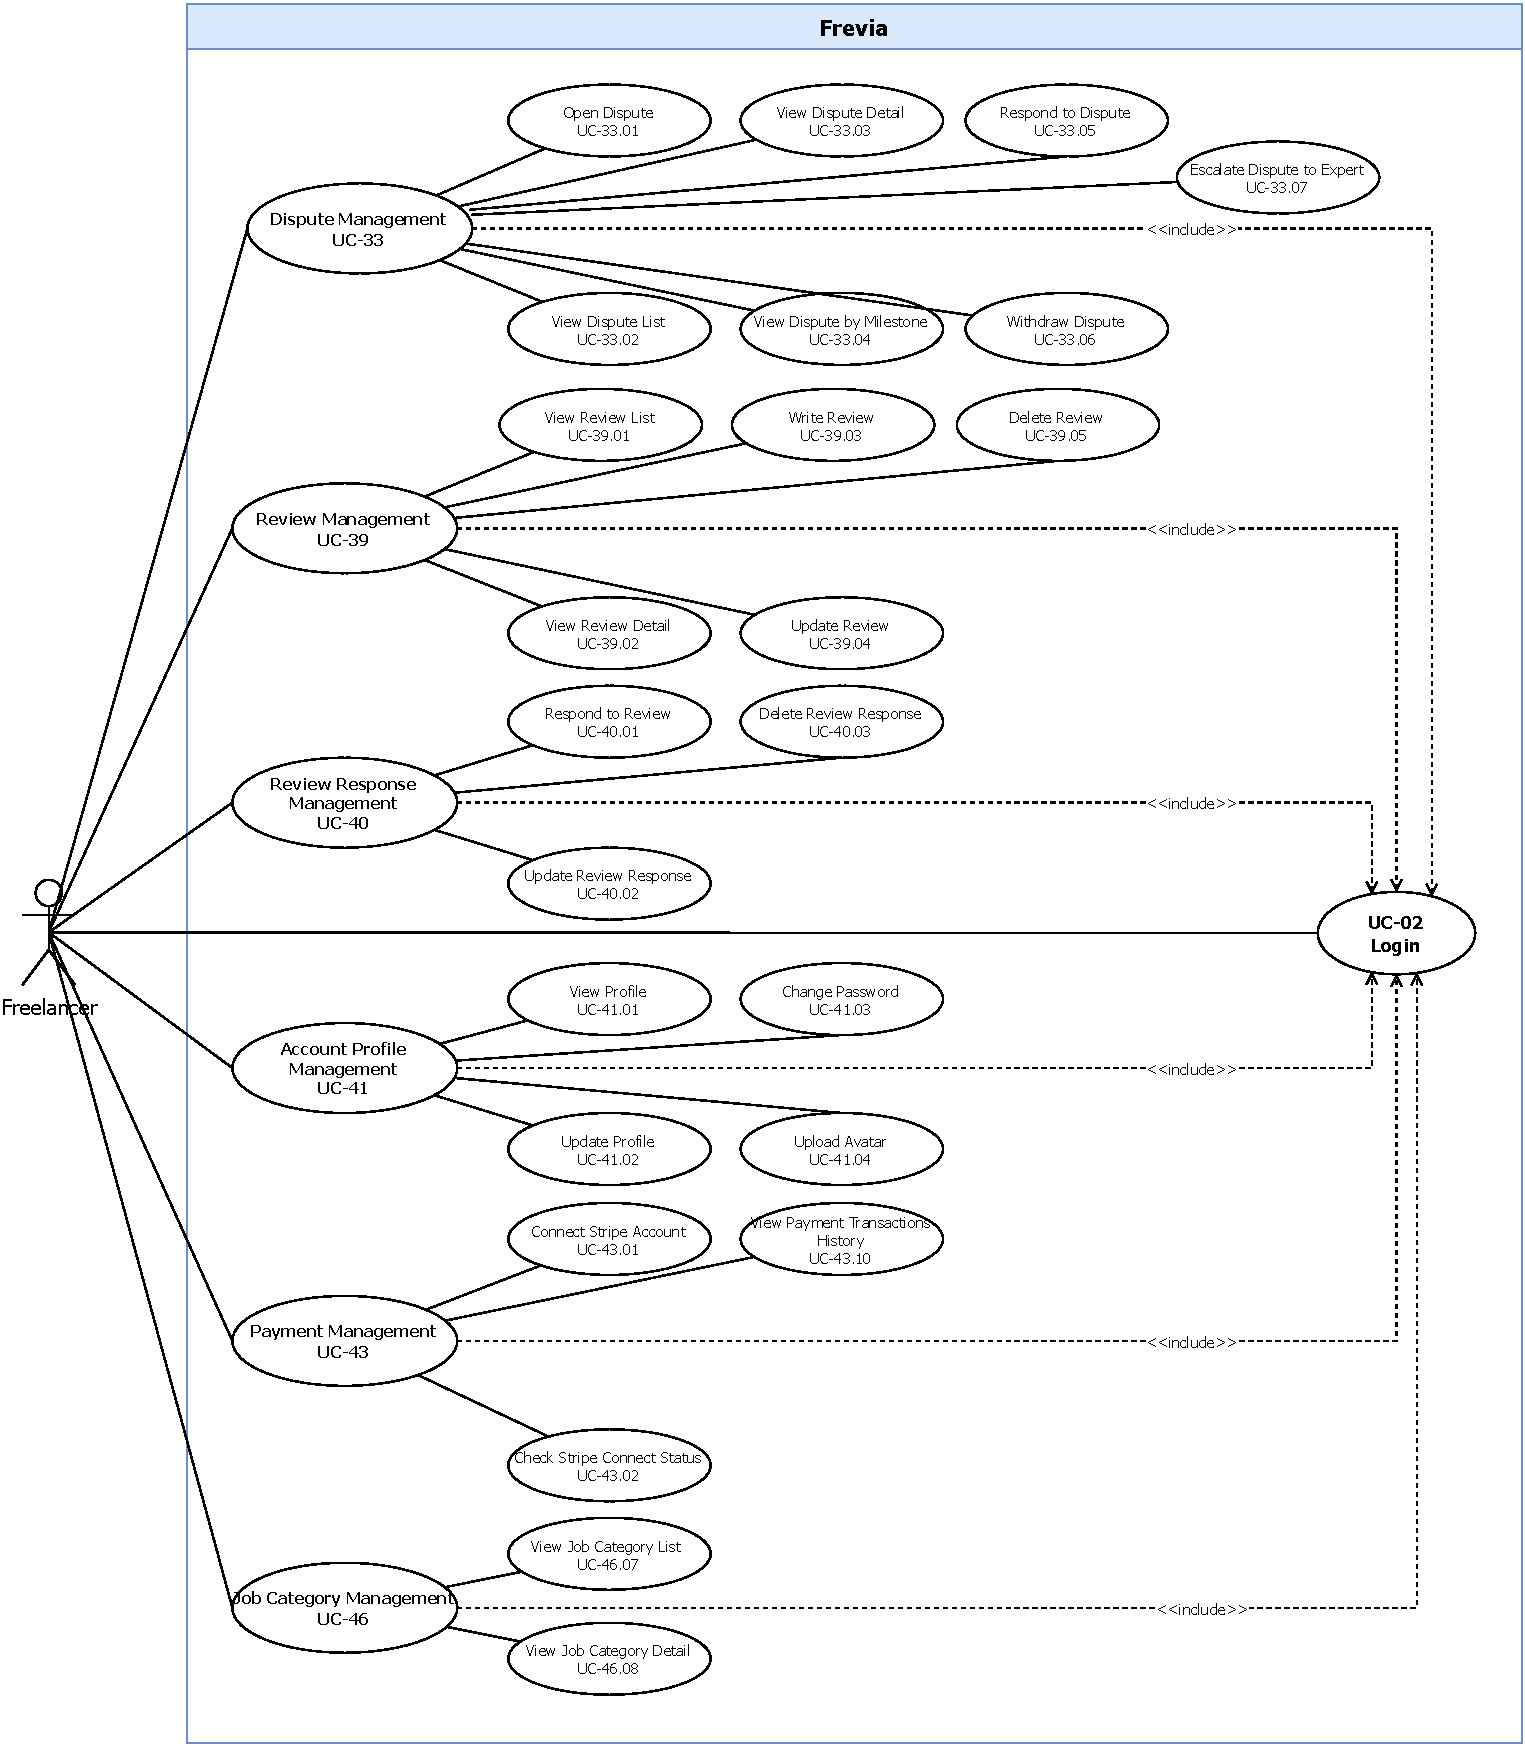
\includegraphics[
        width=\textwidth,
        height=0.85\textheight,
        keepaspectratio
    ]{image/UC_diagram/Freelancer_7.pdf}
    \caption{Freelancer Usecase 7/7}
    \label{fig:uc_freelancer_7}
\end{figure}

% =========================================================================
% 4. Admin Use Case Diagrams
% =========================================================================
\begin{figure}[H]
    \centering
    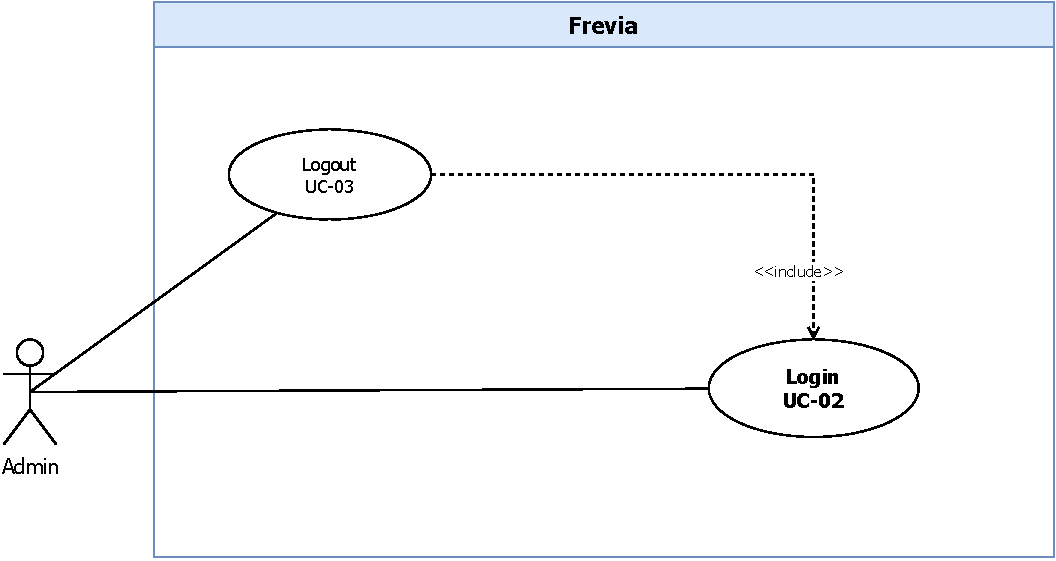
\includegraphics[
        width=\textwidth,
        height=0.85\textheight,
        keepaspectratio
    ]{image/UC_diagram/Admin_1.pdf}
    \caption{Admin Usecase 1/4}
    \label{fig:uc_admin_1}
\end{figure}

\begin{figure}[H]
    \centering
    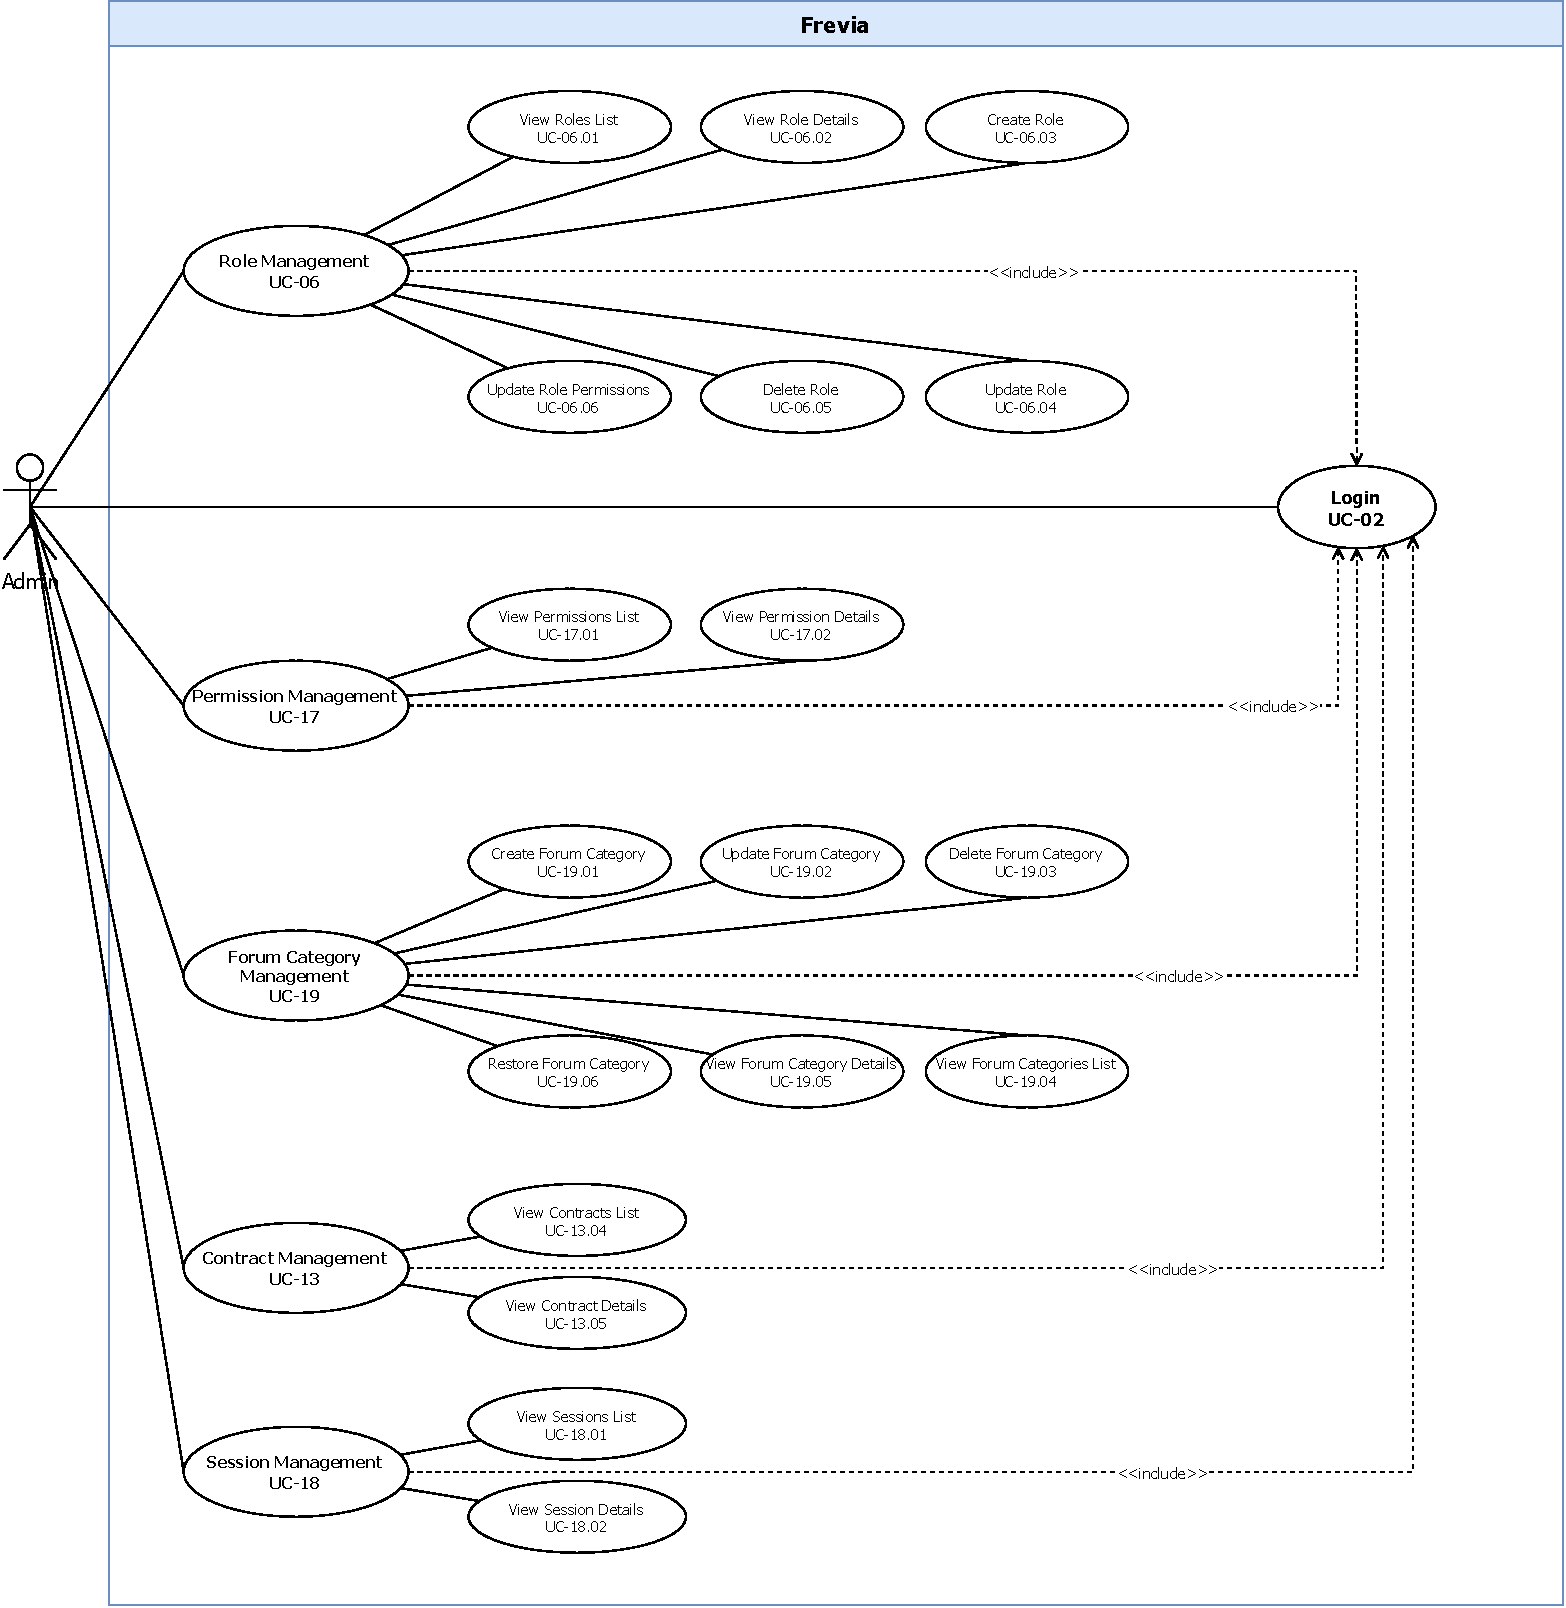
\includegraphics[
        width=\textwidth,
        height=0.85\textheight,
        keepaspectratio
    ]{image/UC_diagram/Admin_2.pdf}
    \caption{Admin Usecase 2/4}
    \label{fig:uc_admin_2}
\end{figure}

\begin{figure}[H]
    \centering
    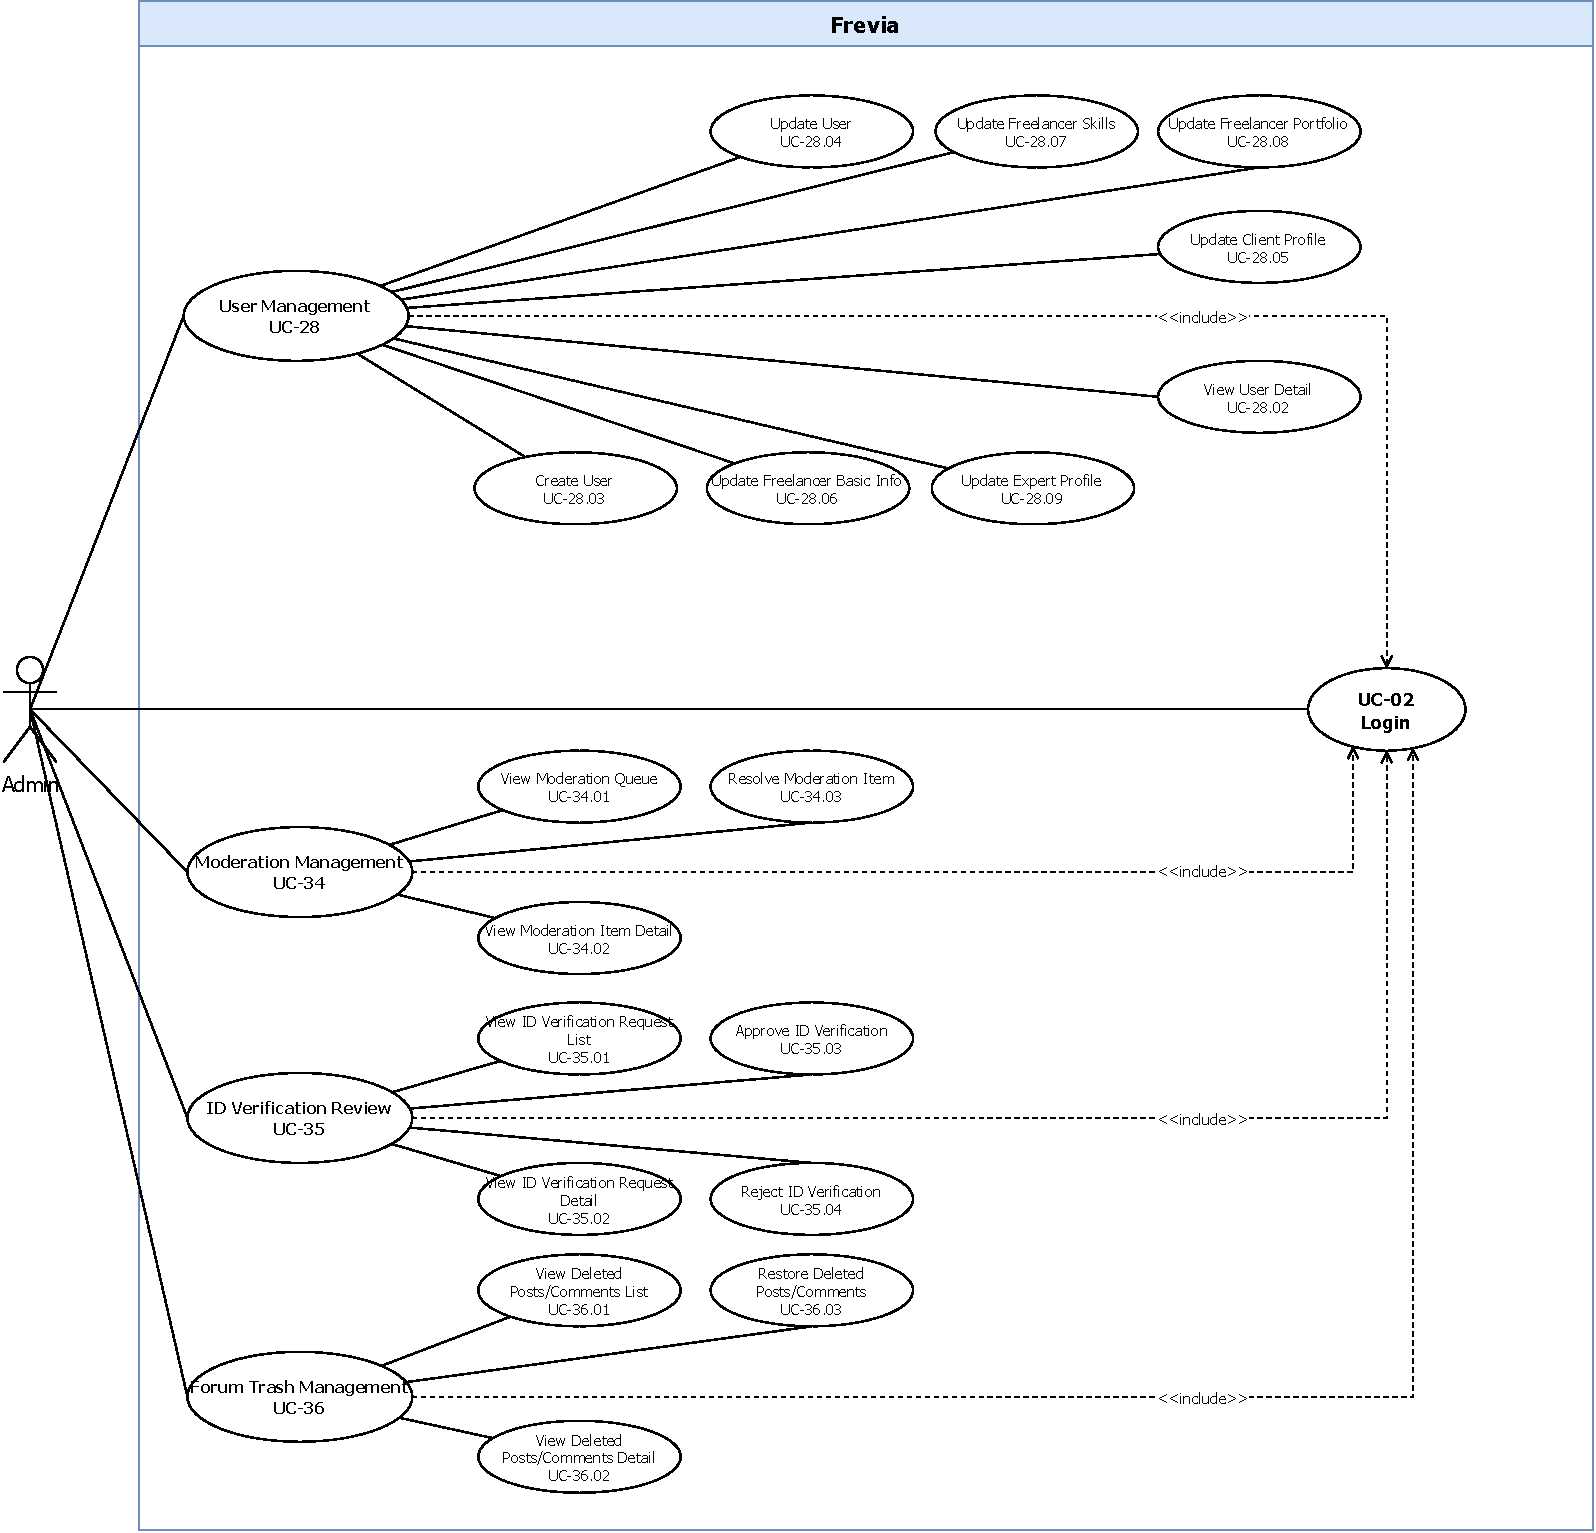
\includegraphics[
        width=\textwidth,
        height=0.85\textheight,
        keepaspectratio
    ]{image/UC_diagram/Admin_3.pdf}
    \caption{Admin Usecase 3/4}
    \label{fig:uc_admin_3}
\end{figure}

\begin{figure}[H]
    \centering
    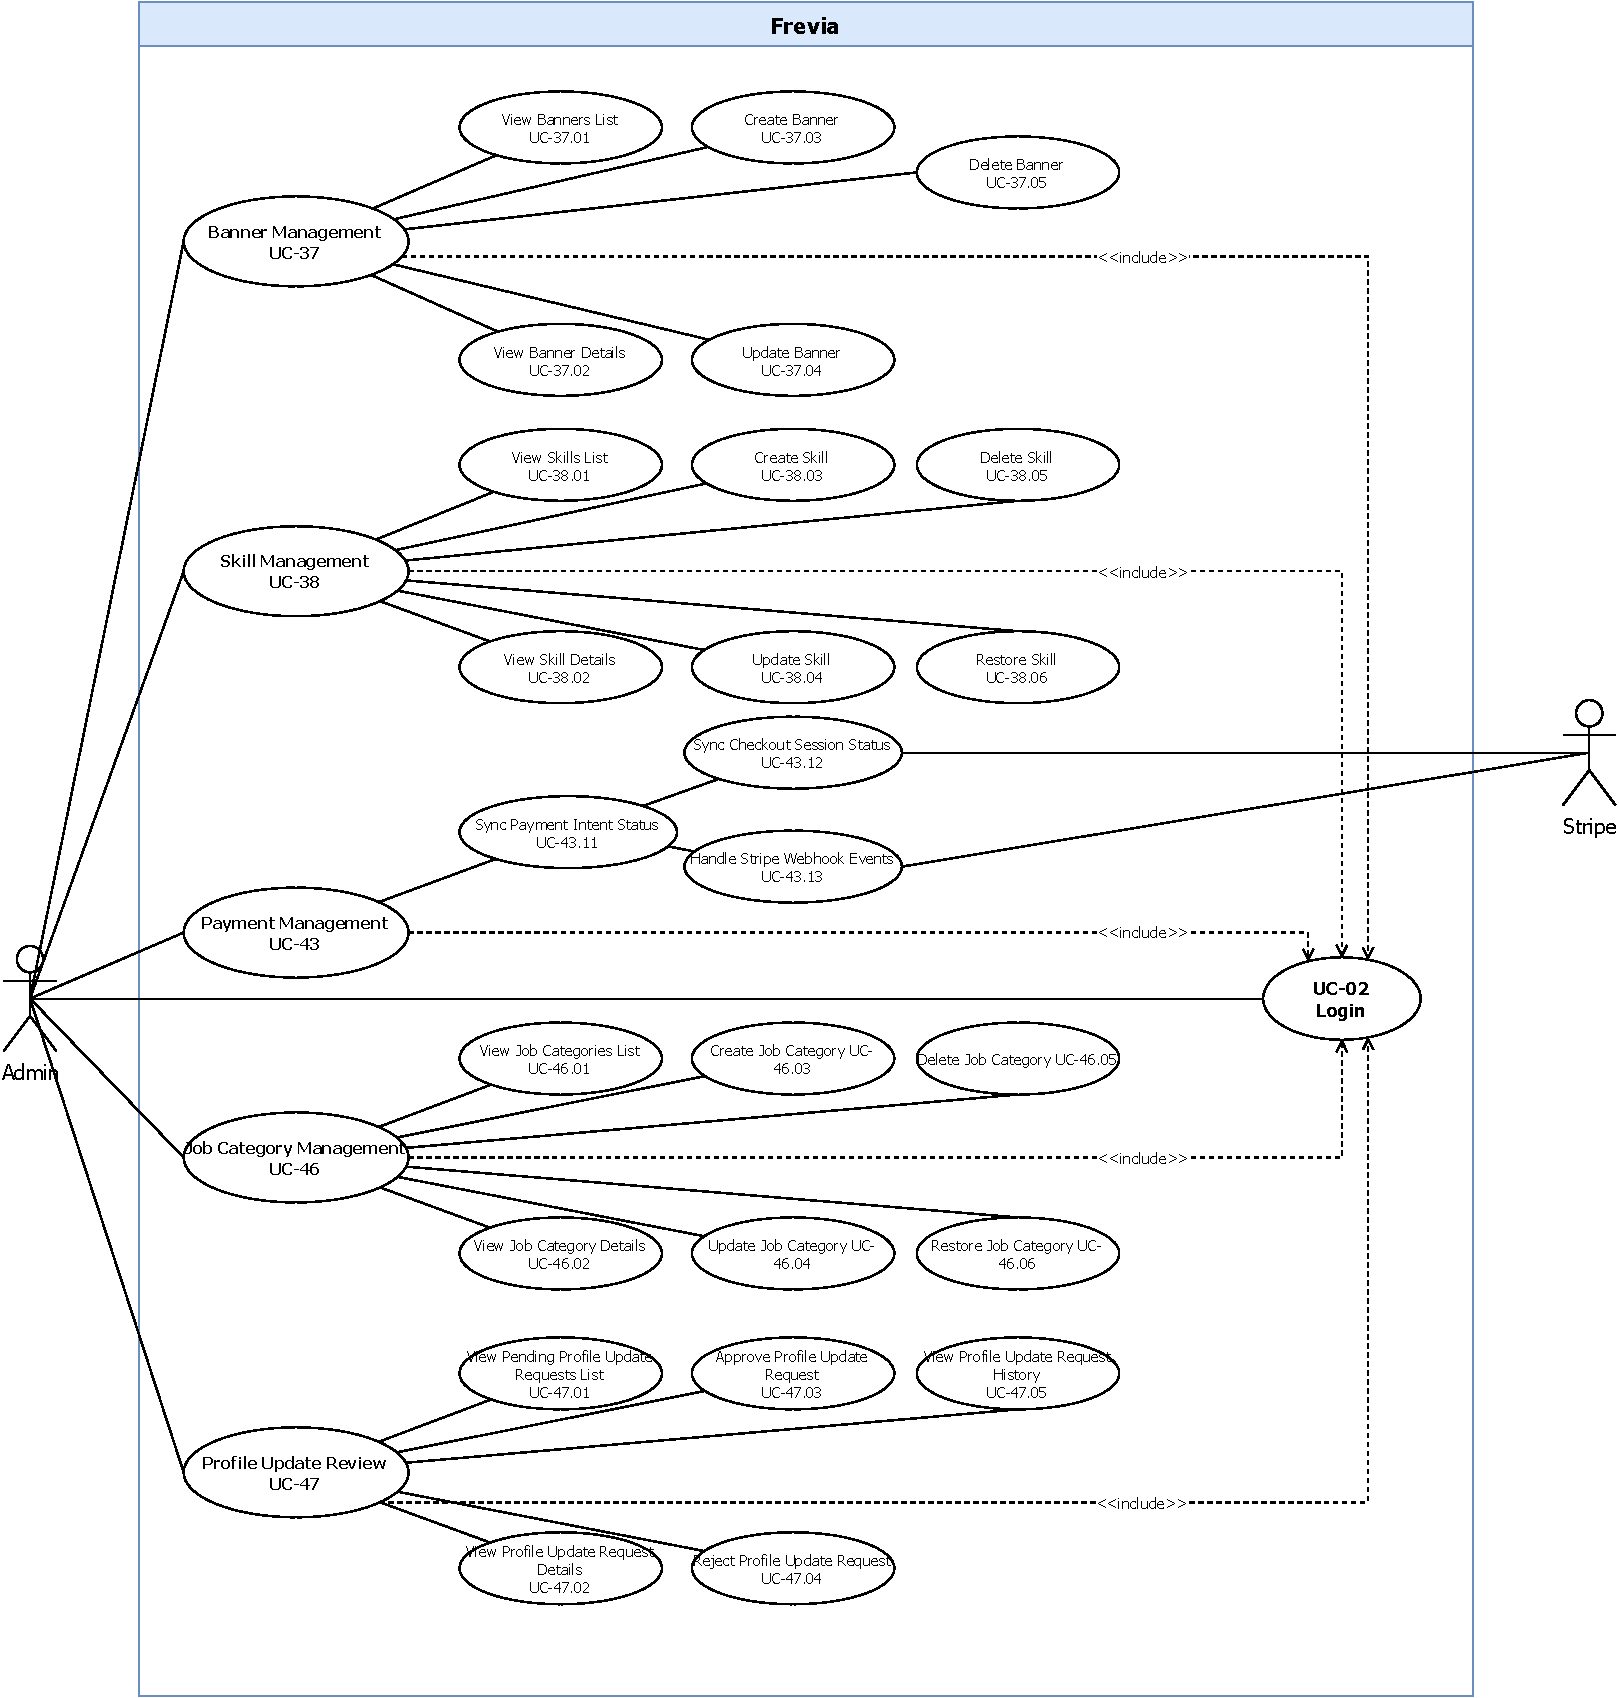
\includegraphics[
        width=\textwidth,
        height=0.85\textheight,
        keepaspectratio
    ]{image/UC_diagram/Admin_4.pdf}
    \caption{Admin Usecase 4/4}
    \label{fig:uc_admin_4}
\end{figure}

% =========================================================================
% 5. Expert Use Case Diagram
% =========================================================================
\begin{figure}[H]
    \centering
    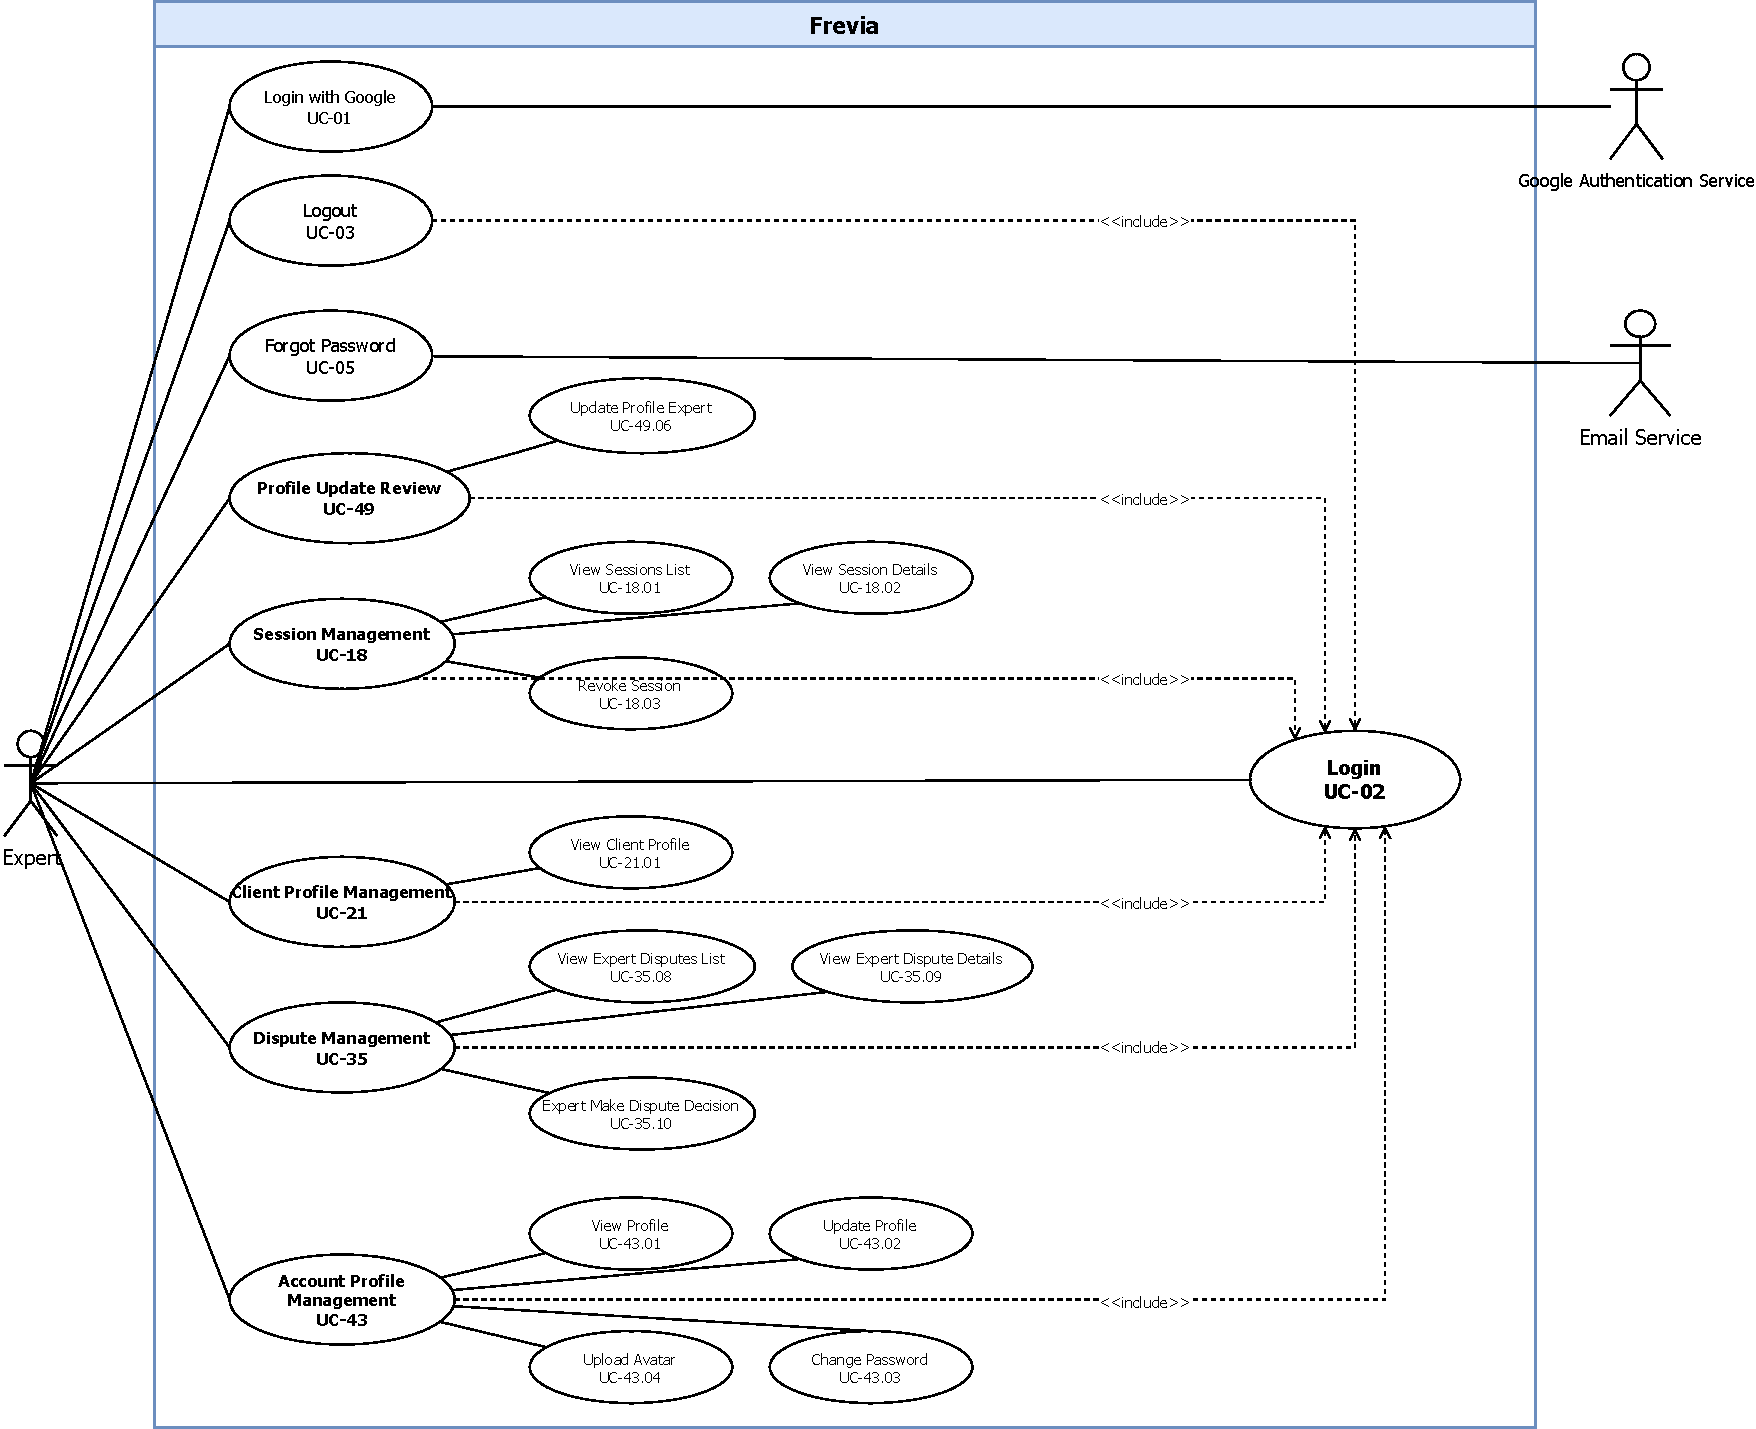
\includegraphics[
        width=\textwidth,
        height=0.85\textheight,
        keepaspectratio
    ]{image/UC_diagram/Expert.pdf}
    \caption{Expert Usecase}
    \label{fig:uc_expert_1}
\end{figure}


\section{Main Use Cases}

Table~\ref{tab:use-case-descriptions} consolidates the core functional use cases of \textbf{Frevia}, specifying each Use Case Identifier, Use Case Name, parent Feature Module, Authorized Actors, and functional summary. Full atomic screen mock-ups, alternative flows, and field validation specifications are preserved in Report 3 (Software Requirement Specification).

\Needspace{12\baselineskip}
\begingroup
\small
\setlength{\tabcolsep}{3.5pt}
\renewcommand{\arraystretch}{1.28}
\begin{longtable}{|C{1.75cm}|C{2.6cm}|C{2.85cm}|C{2.3cm}|L{5.2cm}|}
\caption{Use case table}
\label{tab:use-case-descriptions} \\
\hhline{|-|-|-|-|-|}
\rowcolor{headerbg}
\textbf{ID} & \textbf{Use Case} & \textbf{Feature} & \textbf{Actors} & \textbf{Use Case Description} \\
\hhline{|-|-|-|-|-|}
\endfirsthead

\caption[]{Use case table \textit{(cont.)}} \\
\hhline{|-|-|-|-|-|}
\rowcolor{headerbg}
\textbf{ID} & \textbf{Use Case} & \textbf{Feature} & \textbf{Actors} & \textbf{Use Case Description} \\
\hhline{|-|-|-|-|-|}
\endhead

\hline
\endfoot

\hline
\endlastfoot

UC-01 & Login with Google & \multirow{19.0}{2.75cm}{\centering\arraybackslash Authentication} & Client,\newline Freelancer,\newline Expert,\newline Admin & Allows users to login/register using Google OAuth. \\*
\hhline{|--|~|--|}\noalign{\penalty10000}
UC-02 & Login &  & Client,\newline Freelancer,\newline Expert,\newline Admin & Allows users to log in using email/password and JWT authentication. \\*
\hhline{|--|~|--|}\noalign{\penalty10000}
UC-03 & Logout &  & Client,\newline Freelancer,\newline Expert,\newline Admin & Allows users to logout and terminate authentication session. \\*
\hhline{|--|~|--|}\noalign{\penalty10000}
UC-04 & Register &  & Guest & Allows users to create new accounts using email and password. \\*
\hhline{|--|~|--|}\noalign{\penalty10000}
UC-05 & Forgot Password &  & Client,\newline Freelancer,\newline Expert & Allows users to request password reset via email verification link. \\
\hline
UC-06.01 & View Roles List & \multirow{15.0}{2.75cm}{\centering\arraybackslash Role Management} & Admin & Retrieve list of all roles along with their assigned permissions. \\*
\hhline{|--|~|--|}\noalign{\penalty10000}
UC-06.02 & View Role Details &  & Admin & View detailed information of a specific role including its permissions. \\*
\hhline{|--|~|--|}\noalign{\penalty10000}
UC-06.03 & Create Role &  & Admin & Create a new role with name, description, and a list of permission IDs. \\*
\hhline{|--|~|--|}\noalign{\penalty10000}
UC-06.04 & Update Role &  & Admin & Update a role's name, description, and replace all assigned permissions. \\*
\hhline{|--|~|--|}\noalign{\penalty10000}
UC-06.05 & Delete Role &  & Admin & Delete a role from the system. \\*
\hhline{|--|~|--|}\noalign{\penalty10000}
UC-06.06 & Update Role Permissions &  & Admin & Assign route access rights to roles. \\
\hline
UC-07.01 & View Freelancer Profile & \multirow{16.3}{2.75cm}{\centering\arraybackslash Freelancer Profile Management} & Freelancer & Retrieve all profile information of a freelancer, including data from both profiles and freelancer\_profiles tables. \\*
\hhline{|--|~|--|}\noalign{\penalty10000}
UC-07.02 & Update Freelancer Profile &  & Freelancer & Update fields such as display\_name, bio, title, education, certifications, languages, availability\_status, etc. \\*
\hhline{|--|~|--|}\noalign{\penalty10000}
UC-07.03 & Upload CV &  & Freelancer & Freelancer uploads a CV file in a supported format and associates it with their profile. \\*
\hhline{|--|~|--|}\noalign{\penalty10000}
UC-07.04 & View CV &  & Freelancer & Freelancer views or downloads their uploaded CV. \\*
\hhline{|--|~|--|}\noalign{\penalty10000}
UC-07.05 & Replace CV &  & Freelancer & Freelancer replaces the existing CV with a new file. \\*
\hhline{|--|~|--|}\noalign{\penalty10000}
UC-07.06 & Delete CV &  & Freelancer & Freelancer removes their uploaded CV from the profile. \\
\hline
UC-08.01 & View Freelancer Skills List & \multirow{7.5}{2.75cm}{\centering\arraybackslash Freelancer Skill Management} & Freelancer & Retrieve the list of skills added by the freelancer. \\*
\hhline{|--|~|--|}\noalign{\penalty10000}
UC-08.02 & Add Freelancer Skill &  & Freelancer & Add a new skill to the freelancer's profile with proficiency level. \\*
\hhline{|--|~|--|}\noalign{\penalty10000}
UC-08.03 & Delete Freelancer Skill &  & Freelancer & Remove a skill from the freelancer's profile (hard delete). \\
\hline
UC-09.01 & View Portfolios List & \multirow{12.5}{2.75cm}{\centering\arraybackslash Portfolio Management} & Freelancer & Retrieve the list of portfolios created by the freelancer. \\*
\hhline{|--|~|--|}\noalign{\penalty10000}
UC-09.02 & Add Portfolio &  & Freelancer & Create a new portfolio entry, with optional media file uploads. \\*
\hhline{|--|~|--|}\noalign{\penalty10000}
UC-09.03 & View Portfolio Details &  & Freelancer & View detailed information of a specific portfolio. \\*
\hhline{|--|~|--|}\noalign{\penalty10000}
UC-09.04 & Update Portfolio &  & Freelancer & Update an existing portfolio's information and/or media. \\*
\hhline{|--|~|--|}\noalign{\penalty10000}
UC-09.05 & Delete Portfolio &  & Freelancer & Remove a portfolio from the freelancer's profile (soft delete). \\
\hline
UC-10.01 & View Jobs List & \multirow{6.6}{2.75cm}{\centering\arraybackslash Job Browsing} & Guest,\newline Client,\newline Freelancer & Retrieve paginated job list with filters (category, budget, skills, status, keywords) and sorting options. \\*
\hhline{|--|~|--|}\noalign{\penalty10000}
UC-10.02 & View Job Details &  & Guest,\newline Client,\newline Freelancer & Get full job details: title, description, budget, skills, client info, proposals count, attachments, timeline. \\
\hline
UC-11.01 & View My Jobs & \multirow{21.4}{2.75cm}{\centering\arraybackslash Job Management} & Client & Retrieve the client's own jobs with pagination, filtering by status, keywords, and sorting. Includes job status, budget, proposals count, and creation date. \\*
\hhline{|--|~|--|}\noalign{\penalty10000}
UC-11.02 & Create Job &  & Client & Create and publish a new job. Required: title, description, budget, category, skills. Client/admin only. \\*
\hhline{|--|~|--|}\noalign{\penalty10000}
UC-11.03 & Publish Job &  & Client & Publish a draft job and make it available for freelancers to view and submit proposals. \\*
\hhline{|--|~|--|}\noalign{\penalty10000}
UC-11.04 & Update Job &  & Client & Edit job fields (title, description, budget, skills, status). Owner/admin only; restricted if active contract exists. \\*
\hhline{|--|~|--|}\noalign{\penalty10000}
UC-11.05 & Delete Job &  & Client & Delete a job after checking active proposals/contracts. Owner/admin only. May use soft delete. \\*
\hhline{|--|~|--|}\noalign{\penalty10000}
UC-11.06 & Close Job &  & Client & Allows clients to close an open job posting that has no active contracts so it no longer receives new proposals. \\*
\hhline{|--|~|--|}\noalign{\penalty10000}
UC-11.07 & Reopen Job &  & Client & Allows clients to reopen a closed or expired job posting within 60 days so it becomes open again. \\
\hline
UC-12.01 & View Bookmarked Jobs List & \multirow{7.5}{2.75cm}{\centering\arraybackslash Bookmarked Jobs Management} & Freelancer & List all jobs bookmarked by user, including job title, budget, client name, bookmark date. \\*
\hhline{|--|~|--|}\noalign{\penalty10000}
UC-12.02 & Bookmark Job &  & Freelancer & Add job to bookmarks. Idempotent; duplicate requests ignored. \\*
\hhline{|--|~|--|}\noalign{\penalty10000}
UC-12.03 & Remove Bookmark &  & Freelancer & Remove bookmark from a job. Returns 404 if not bookmarked. \\
\hline
UC-13.01 & Create Contract & \multirow{16.7}{2.75cm}{\centering\arraybackslash Contract Management (Part 1)} & Client & Insert into contracts (job\_id, client\_id, freelancer\_id, terms, total\_amount, deposit\_percent). \\*
\hhline{|--|~|--|}\noalign{\penalty10000}
UC-13.02 & Update Contract &  & Client & Update terms, total\_amount, deposit\_percent of a contract before signing. \\*
\hhline{|--|~|--|}\noalign{\penalty10000}
UC-13.03 & Complete Contract &  & Client & Mark contract COMPLETED after all milestones done. \\*
\hhline{|--|~|--|}\noalign{\penalty10000}
UC-13.04 & View Contracts List &  & Client,\newline Freelancer,\newline Admin & Get all contracts where user is client or freelancer (contracts table). \\*
\hhline{|--|~|--|}\noalign{\penalty10000}
UC-13.05 & View Contract Details &  & Client,\newline Freelancer,\newline Admin & Get contract details: terms, total\_amount, deposit\_percent, status, signatures, milestones. \\*
\hhline{|--|~|--|}\noalign{\penalty10000}
UC-13.06 & Sign Contract &  & Client,\newline Freelancer & Set signed\_by\_client or signed\_by\_freelancer = true. \\
\hline
UC-13.07 & Export Contract PDF & \multirow{15.0}{2.75cm}{\centering\arraybackslash Contract Management (Part 2)} & Client,\newline Freelancer,\newline Admin & Generates and exports contract terms, clauses, and signatures into a downloadable PDF document. \\*
\hhline{|--|~|--|}\noalign{\penalty10000}
UC-13.08 & Cancel Contract &  & Client,\newline Freelancer & Allows either party to cancel or terminate a contract prior to completion. \\*
\hhline{|--|~|--|}\noalign{\penalty10000}
UC-13.09 & View Contract Files &  & Client,\newline Freelancer & List files from shared\_files for a contract. \\*
\hhline{|--|~|--|}\noalign{\penalty10000}
UC-13.10 & Upload Contract File &  & Client,\newline Freelancer & Insert into shared\_files (file\_url, file\_name). \\*
\hhline{|--|~|--|}\noalign{\penalty10000}
UC-13.11 & Delete Contract File &  & Client,\newline Freelancer & Soft-delete file (set deleted\_at). \\*
\hhline{|--|~|--|}\noalign{\penalty10000}
UC-13.12 & Reject Contract Offer &  & Freelancer & Freelancer rejects contract proposal with mandatory reason \\
\hline
UC-14.01 & View Forum Categories List & \multirow{5.0}{2.75cm}{\centering\arraybackslash Forum Browsing} & Client,\newline Freelancer & Retrieve all forum categories (forum\_categories: name, description). \\*
\hhline{|--|~|--|}\noalign{\penalty10000}
UC-14.02 & View Forum Category Details &  & Client,\newline Freelancer & Get a single category by ID. \\
\hline
UC-15.01 & View Posts List & \multirow{10.0}{2.75cm}{\centering\arraybackslash Forum Post Management (Part 1)} & Client,\newline Freelancer & Get paginated list of forum posts (forum\_posts) with optional category filter. \\*
\hhline{|--|~|--|}\noalign{\penalty10000}
UC-15.02 & View Post Details &  & Client,\newline Freelancer & Get full post details: title, content, author, category, created\_at. \\*
\hhline{|--|~|--|}\noalign{\penalty10000}
UC-15.03 & Create Post &  & Client,\newline Freelancer & Insert new post into forum\_posts (title, content, category\_id). \\*
\hhline{|--|~|--|}\noalign{\penalty10000}
UC-15.04 & Update Post &  & Client,\newline Freelancer & Update a post's title, content, or category. Only the author can edit. \\
\hline
UC-15.05 & Delete Post & \multirow{10.0}{2.75cm}{\centering\arraybackslash Forum Post Management (Part 2)} & Client,\newline Freelancer & Soft-delete a post (set deleted\_at). \\*
\hhline{|--|~|--|}\noalign{\penalty10000}
UC-15.06 & Like Post &  & Client,\newline Freelancer & Insert a like record into forum\_likes (user\_id, post\_id, reaction\_type). \\*
\hhline{|--|~|--|}\noalign{\penalty10000}
UC-15.07 & Unlike Post &  & Client,\newline Freelancer & Remove the like record from forum\_likes for the user and post. \\*
\hhline{|--|~|--|}\noalign{\penalty10000}
UC-15.08 & View Post Likes &  & Client,\newline Freelancer & Get list of users like this post. \\
\hline
UC-16.01 & View Post Comments & \multirow{17.9}{2.75cm}{\centering\arraybackslash Forum Comment Management} & Client,\newline Freelancer & Get list of comments for a post (forum\_comments: content, author, created\_at). \\*
\hhline{|--|~|--|}\noalign{\penalty10000}
UC-16.02 & Create Comment &  & Client,\newline Freelancer & Insert a new comment into forum\_comments (post\_id, user\_id, content). \\*
\hhline{|--|~|--|}\noalign{\penalty10000}
UC-16.03 & Update Comment &  & Client,\newline Freelancer & Update a comment's content. Only comment owner can edit. \\*
\hhline{|--|~|--|}\noalign{\penalty10000}
UC-16.04 & Delete Comment &  & Client,\newline Freelancer & Soft-delete a comment (set deleted\_at). \\*
\hhline{|--|~|--|}\noalign{\penalty10000}
UC-16.05 & Like Comment &  & Client,\newline Freelancer & Insert a like record into forum\_likes (user\_id, comment\_id, reaction\_type). \\*
\hhline{|--|~|--|}\noalign{\penalty10000}
UC-16.06 & Unlike Comment &  & Client,\newline Freelancer & Remove the like record for that user and comment. \\*
\hhline{|--|~|--|}\noalign{\penalty10000}
UC-16.07 & Report Content &  & Client,\newline Freelancer & Insert a report into forum\_reports (reporter\_id, post\_id/comment\_id, reason). Status defaults to PENDING. \\
\hline
UC-17.01 & View Permissions List & \multirow{5.0}{2.75cm}{\centering\arraybackslash Permission Management} & Admin & Retrieve all permissions (id, name, path, method, module) for admin to assign to roles. \\*
\hhline{|--|~|--|}\noalign{\penalty10000}
UC-17.02 & View Permission Details &  & Admin & View detailed information of a specific permission. \\
\hline
UC-18.01 & View Sessions List & \multirow{12.1}{2.75cm}{\centering\arraybackslash Session Management} & Client,\newline Freelancer,\newline Expert,\newline Admin & View a list of active login sessions. \\*
\hhline{|--|~|--|}\noalign{\penalty10000}
UC-18.02 & View Session Details &  & Client,\newline Freelancer,\newline Expert,\newline Admin & View login session information (device, IP address, login time, approximate location, etc.) \\*
\hhline{|--|~|--|}\noalign{\penalty10000}
UC-18.03 & Revoke Session &  & Client,\newline Freelancer,\newline Expert & Log out of a specific device remotely. \\
\hline
UC-19.01 & Create Forum Category & \multirow{15.0}{2.75cm}{\centering\arraybackslash Forum Category Management} & Admin & Allows admins to create a new forum category. \\*
\hhline{|--|~|--|}\noalign{\penalty10000}
UC-19.02 & Update Forum Category &  & Admin & Allows admins to update an existing forum category. \\*
\hhline{|--|~|--|}\noalign{\penalty10000}
UC-19.03 & Delete Forum Category &  & Admin & Allows admins to soft-delete a forum category. \\*
\hhline{|--|~|--|}\noalign{\penalty10000}
UC-19.04 & View Forum Categories List &  & Admin & Allows admins to view the list of forum categories. \\*
\hhline{|--|~|--|}\noalign{\penalty10000}
UC-19.05 & View Forum Category Details &  & Admin & Allows admins to view the details of a specific forum category. \\*
\hhline{|--|~|--|}\noalign{\penalty10000}
UC-19.06 & Restore Forum Category &  & Admin & Restore a deleted Category forum by setting deletedAt back to null. \\
\hline
UC-20.01 & Upload Identity Documents & \multirow{5.1}{2.75cm}{\centering\arraybackslash Identity Verification} & Freelancer & Upload identification documents (ID card, passport, etc.) for freelancer identity verification. \\*
\hhline{|--|~|--|}\noalign{\penalty10000}
UC-20.02 & View Verification Status &  & Freelancer & Get the current status of the identity verification process (pending, approved, rejected). \\
\hline
UC-21.01 & View Client Profile & \multirow{7.3}{2.75cm}{\centering\arraybackslash Client Profile Management} & Client,\newline Freelancer,\newline Expert,\newline Admin & Retrieve detailed client profile information (company name, description, website, etc.) by client user ID. \\*
\hhline{|--|~|--|}\noalign{\penalty10000}
UC-21.02 & Update Company Information &  & Client & Update company-related information (name, description, website) for the currently authenticated client. \\
\hline
UC-22.01 & View Social Links List & \multirow{7.5}{2.75cm}{\centering\arraybackslash Social Links} & Client,\newline Freelancer & Retrieve all social links of the authenticated user. \\*
\hhline{|--|~|--|}\noalign{\penalty10000}
UC-22.02 & Add Social Link &  & Client,\newline Freelancer & Add a new social link to the user's profile. \\*
\hhline{|--|~|--|}\noalign{\penalty10000}
UC-22.03 & Delete Social Link &  & Client,\newline Freelancer & Remove a social link from the user's profile. \\
\hline
UC-23.01 & View Favorite Freelancers List & \multirow{7.5}{2.75cm}{\centering\arraybackslash Favorites} & Client & Get the list of freelancers marked as favorites by the user. \\*
\hhline{|--|~|--|}\noalign{\penalty10000}
UC-23.02 & Add Freelancer to Favorites &  & Client & Add a freelancer to the user's favorites list. \\*
\hhline{|--|~|--|}\noalign{\penalty10000}
UC-23.03 & Remove Freelancer from Favorites &  & Client & Remove a freelancer from the user's favorites list. \\
\hline
UC-24.01 & View Saved Searches List & \multirow{10.0}{2.75cm}{\centering\arraybackslash Saved Search Management} & Freelancer & Retrieve all saved job search filters with labels and filter criteria. \\*
\hhline{|--|~|--|}\noalign{\penalty10000}
UC-24.02 & View Saved Search Details &  & Freelancer & Get details of a saved search: label, filters (keywords, category, skills, budget). \\*
\hhline{|--|~|--|}\noalign{\penalty10000}
UC-24.03 & Create Saved Search &  & Freelancer & Save current search parameters as a named filter for quick reuse. \\*
\hhline{|--|~|--|}\noalign{\penalty10000}
UC-24.04 & Delete Saved Search &  & Freelancer & Permanently delete a saved search. \\
\hline
UC-25.01 & View Job Alerts List & \multirow{13.1}{2.75cm}{\centering\arraybackslash Job Alert Management} & Freelancer & List all job alerts with criteria, frequency (daily/weekly/instant), and notification channel. \\*
\hhline{|--|~|--|}\noalign{\penalty10000}
UC-25.02 & View Job Alert Details &  & Freelancer & View alert configuration: filters, frequency, active status, last triggered time. \\*
\hhline{|--|~|--|}\noalign{\penalty10000}
UC-25.03 & Create Job Alert &  & Freelancer & Create alert with criteria, frequency, and delivery channel. System auto-sends matching job notifications. \\*
\hhline{|--|~|--|}\noalign{\penalty10000}
UC-25.04 & Update Job Alert &  & Freelancer & Update alert: criteria, frequency, channels, on/off. Only owner. \\*
\hhline{|--|~|--|}\noalign{\penalty10000}
UC-25.05 & Delete Job Alert &  & Freelancer & Permanently delete alert. Stops all future notifications. \\
\hline
UC-26.01 & View Milestones List & \multirow{17.0}{2.75cm}{\centering\arraybackslash Contract Milestones} & Client,\newline Freelancer & Retrieve all milestones of a contract, including title, amount, due date, and current status. \\*
\hhline{|--|~|--|}\noalign{\penalty10000}
UC-26.02 & View Milestone Details &  & Client,\newline Freelancer & Retrieve detailed information of a specific milestone, including its amount, due date, status, and related files and submissions. \\*
\hhline{|--|~|--|}\noalign{\penalty10000}
UC-26.03 & Create Milestone &  & Client & Create a new milestone for a contract with a title, description, amount, and due date. \\*
\hhline{|--|~|--|}\noalign{\penalty10000}
UC-26.04 & Update Milestone &  & Client & Update milestone information such as title, description, amount, and due date before the milestone is accepted. \\*
\hhline{|--|~|--|}\noalign{\penalty10000}
UC-26.05 & Delete Milestone &  & Client & Delete a milestone that has not yet been accepted by the freelancer. \\*
\hhline{|--|~|--|}\noalign{\penalty10000}
UC-26.06 & Update Milestone Progress &  & Freelancer & Allow the freelancer to accept a pending milestone and confirm their agreement to perform the work. \\
\hline
UC-27.01 & View Milestone Files & \multirow{7.8}{2.75cm}{\centering\arraybackslash Milestone File Management} & Client,\newline Freelancer & Retrieve all files associated with a milestone and allow authorized users to view or download them. \\*
\hhline{|--|~|--|}\noalign{\penalty10000}
UC-27.02 & Upload Milestone File &  & Freelancer & Allow the freelancer to upload deliverable files for a milestone before submitting the work. \\*
\hhline{|--|~|--|}\noalign{\penalty10000}
UC-27.03 & Delete Milestone File &  & Freelancer & Allow the freelancer to delete an uploaded milestone file before it is submitted. \\
\hline
UC-28.01 & Submit Milestone & \multirow{16.5}{2.75cm}{\centering\arraybackslash Milestone Submission} & Freelancer & Allow the freelancer to submit a completed milestone with a note and selected deliverable files for client review. \\*
\hhline{|--|~|--|}\noalign{\penalty10000}
UC-28.02 & View Milestone Submissions List &  & Client & Retrieve the latest milestone submission and submission history, including notes, files, status, and submission timestamps. \\*
\hhline{|--|~|--|}\noalign{\penalty10000}
UC-28.03 & View Milestone Submission Details &  & Client & Retrieve the latest milestone submission detail and submission history, including notes, files, status, and submission timestamps. \\*
\hhline{|--|~|--|}\noalign{\penalty10000}
UC-28.04 & Request Milestone Changes &  & Client & Allow the client to request changes to a submitted milestone and provide feedback or revision instructions. \\*
\hhline{|--|~|--|}\noalign{\penalty10000}
UC-28.05 & Approve Milestone &  & Client & Approve a submitted milestone after reviewing the deliverables and confirm that the milestone is completed successfully. \\
\hline
UC-29.01 & View Conversations List & \multirow{13.6}{2.75cm}{\centering\arraybackslash Conversation Management (Part 1)} & Client,\newline Freelancer & Get all conversations for current user (conversations with participant\_1, participant\_2). Each includes last message preview and unread count. \\*
\hhline{|--|~|--|}\noalign{\penalty10000}
UC-29.02 & Start Conversation &  & Client,\newline Freelancer & Create new conversation between two users (participant\_1, participant\_2). Returns existing conversation if already exists (unique constraint). \\*
\hhline{|--|~|--|}\noalign{\penalty10000}
UC-29.03 & View Conversation Details &  & Client,\newline Freelancer & Get a conversation's full message list (direct\_messages ordered by created\_at). Includes sender info, read status. \\*
\hhline{|--|~|--|}\noalign{\penalty10000}
UC-29.04 & Send Message &  & Client,\newline Freelancer & Insert a new message into direct\_messages (sender\_id, message) for the conversation. \\
\hline
UC-29.05 & Mark Message as Read & \multirow{10.1}{2.75cm}{\centering\arraybackslash Conversation Management (Part 2)} & Client,\newline Freelancer & Set is\_read = true for a specific message (direct\_messages). \\*
\hhline{|--|~|--|}\noalign{\penalty10000}
UC-29.06 & Delete/Recall Message &  & Client,\newline Freelancer & Soft-delete a message (set deleted\_at in direct\_messages). The message becomes hidden in UI. \\*
\hhline{|--|~|--|}\noalign{\penalty10000}
UC-29.07 & Pin/Unpin Conversation &  & Client,\newline Freelancer & Pin or Unpin the conversation. \\*
\hhline{|--|~|--|}\noalign{\penalty10000}
UC-29.08 & Send File &  & Client,\newline Freelancer & Send a file to the other participant such as docx, excel, pdf, ... etc \\
\hline
UC-30.01 & View Users List & \multirow{14.9}{2.75cm}{\centering\arraybackslash User Management (Part 1)} & Admin & Allows admin to view, search, filter and sort all user accounts, filterable by role (Client/Freelancer/Admin/Custom role). \\*
\hhline{|--|~|--|}\noalign{\penalty10000}
UC-30.02 & View User Details &  & Admin & Retrieve general account information plus separate tabs for each role profile the user currently holds. \\*
\hhline{|--|~|--|}\noalign{\penalty10000}
UC-30.03 & Create User &  & Admin & Allows admin to create a new account and select initial role(s) to activate (Client/Freelancer/Custom role). \\*
\hhline{|--|~|--|}\noalign{\penalty10000}
UC-30.04 & Update User &  & Admin & Allows admin to edit general account information (email, status, etc.). \\*
\hhline{|--|~|--|}\noalign{\penalty10000}
UC-30.05 & Update Client Profile &  & Admin & Within the User Detail screen, allows admin to edit the Client profile tab (company name, description, website). \\
\hline
UC-30.06 & Update Freelancer Basic Info & \multirow{10.0}{2.75cm}{\centering\arraybackslash User Management (Part 2)} & Admin & Edit professional title, bio, languages/education/certifications (string list). \\*
\hhline{|--|~|--|}\noalign{\penalty10000}
UC-30.07 & Update Freelancer Skills &  & Admin & Select a skill from the catalog (Select) + level 1–10; save by replacing the list. \\*
\hhline{|--|~|--|}\noalign{\penalty10000}
UC-30.08 & Update Freelancer Portfolio &  & Admin & Add/edit/delete (soft-delete) portfolio items (title/description/technologies/projectUrl). \\*
\hhline{|--|~|--|}\noalign{\penalty10000}
UC-30.09 & Update Expert Profile &  & Admin & Edit expert profile on the admin page. \\
\hline
UC-31.01 & View Following List & \multirow{7.5}{2.75cm}{\centering\arraybackslash Following} & Client & Get the list of freelancers the user is following. \\*
\hhline{|--|~|--|}\noalign{\penalty10000}
UC-31.02 & Follow Freelancer &  & Client & Start following a freelancer. \\*
\hhline{|--|~|--|}\noalign{\penalty10000}
UC-31.03 & Unfollow Freelancer &  & Client & Stop following a freelancer. \\
\hline
UC-32.01 & View Notifications List & \multirow{10.7}{2.75cm}{\centering\arraybackslash Notification Management} & Client,\newline Freelancer & Get all notifications for current user (notifications table) with type, title, message, data, is\_read, created\_at. \\*
\hhline{|--|~|--|}\noalign{\penalty10000}
UC-32.02 & Mark Notification as Read &  & Client,\newline Freelancer & Set is\_read = true for a specific notification (notifications). \\*
\hhline{|--|~|--|}\noalign{\penalty10000}
UC-32.03 & Mark All Notifications as Read &  & Client,\newline Freelancer & Bulk update: set is\_read = true for all unread notifications of the current user. \\*
\hhline{|--|~|--|}\noalign{\penalty10000}
UC-32.04 & Delete Notification &  & Client,\newline Freelancer & Soft-delete a notification (set deleted\_at). \\
\hline
UC-33.01 & Switch Role & \multirow{10.4}{2.75cm}{\centering\arraybackslash Account Management} & Client,\newline Freelancer & Allows users who hold both Client and Freelancer roles to switch their active working context between the two roles within the same account without logging out and back in. \\*
\hhline{|--|~|--|}\noalign{\penalty10000}
UC-33.02 & Join New Role &  & Client,\newline Freelancer & Allows users with a primary role to add the missing complementary role. The new role becomes the primary role, a new JWT is issued immediately, and role switching is enabled without requiring re-login. \\
\hline
UC-34.01 & View My Proposals List & \multirow{16.8}{2.75cm}{\centering\arraybackslash Proposal Management (Part 1)} & Freelancer & Freelancer retrieves list of all proposals they have submitted across jobs, with status (pending, accepted, rejected, withdrawn). \\*
\hhline{|--|~|--|}\noalign{\penalty10000}
UC-34.02 & View My Proposal Details &  & Freelancer & Freelancer views the full details of their submitted proposal, including cover letter, bid amount, estimated duration, attachments, job information, and current status. \\*
\hhline{|--|~|--|}\noalign{\penalty10000}
UC-34.03 & Submit Proposal &  & Freelancer & Freelancer submits a proposal for a job: cover letter, bid amount, estimated duration, optional attachments. \\*
\hhline{|--|~|--|}\noalign{\penalty10000}
UC-34.04 & Update Proposal &  & Freelancer & Freelancer updates proposal details (cover letter, bid, duration) only when status is PENDING. \\*
\hhline{|--|~|--|}\noalign{\penalty10000}
UC-34.05 & Withdraw Proposal &  & Freelancer & Freelancer withdraws a submitted proposal (status becomes WITHDRAWN). Cannot withdraw if already accepted. \\
\hline
UC-34.06 & Accept Proposal & \multirow{12.9}{2.75cm}{\centering\arraybackslash Proposal Management (Part 2)} & Client & Client accepts a freelancer's proposal, changing status to ACCEPTED. May trigger contract creation. \\*
\hhline{|--|~|--|}\noalign{\penalty10000}
UC-34.07 & Reject Proposal &  & Client & Client rejects a proposal, status becomes REJECTED. Optionally provide a reason. \\*
\hhline{|--|~|--|}\noalign{\penalty10000}
UC-34.08 & View Job Proposals List &  & Client & Client retrieves all proposals submitted for a specific job, including freelancer info, bid amount, cover letter, status. \\*
\hhline{|--|~|--|}\noalign{\penalty10000}
UC-34.09 & View Proposal Details &  & Client & View full detail of a proposal: cover letter, bid amount, estimated duration, freelancer profile, attachments. Accessible by job owner or proposal owner. \\
\hline
UC-35.01 & Open Dispute & \multirow{15.0}{2.75cm}{\centering\arraybackslash Dispute Management (Part 1)} & Client,\newline Freelancer & Open a new dispute ticket with reason and proposed split amount \\*
\hhline{|--|~|--|}\noalign{\penalty10000}
UC-35.02 & View Disputes List &  & Client,\newline Freelancer & View paginated list of disputes where user is a participant \\*
\hhline{|--|~|--|}\noalign{\penalty10000}
UC-35.03 & View Dispute Details &  & Client,\newline Freelancer & View full dispute details, proposed split, evidence files and timeline \\*
\hhline{|--|~|--|}\noalign{\penalty10000}
UC-35.04 & View Dispute by Milestone &  & Client,\newline Freelancer & Query current active dispute associated with a milestone ID \\*
\hhline{|--|~|--|}\noalign{\penalty10000}
UC-35.05 & Respond to Dispute &  & Client,\newline Freelancer & Counterparty accepts or declines proposed escrow split resolution \\*
\hhline{|--|~|--|}\noalign{\penalty10000}
UC-35.06 & Withdraw Dispute &  & Client,\newline Freelancer & Dispute opener cancels and withdraws dispute ticket \\
\hline
UC-35.07 & Escalate Dispute to Expert & \multirow{13.1}{2.75cm}{\centering\arraybackslash Dispute Management (Part 2)} & Client,\newline Freelancer & Escalate dispute directly to Frevia Expert when mutually declined or expired \\*
\hhline{|--|~|--|}\noalign{\penalty10000}
UC-35.08 & View Expert Disputes List &  & Expert & Expert views list of escalated disputes requiring arbitration \\*
\hhline{|--|~|--|}\noalign{\penalty10000}
UC-35.09 & View Expert Dispute Details &  & Expert & Expert views dispute evidence, contract history and conversation \\*
\hhline{|--|~|--|}\noalign{\penalty10000}
UC-35.10 & Expert Make Dispute Decision &  & Expert & Expert issues binding split decision and executes automatic escrow settlement \\*
\hhline{|--|~|--|}\noalign{\penalty10000}
UC-35.11 & Upload Dispute Evidence File &  & Client,\newline Freelancer & Upload evidence files for dispute resolution and store file metadata, including URL, file name, size, and type \\
\hline
UC-36.01 & View Moderation Queue & \multirow{7.9}{2.75cm}{\centering\arraybackslash Moderation Management} & Admin & Get list of moderation items from moderation\_queue (content\_type, content\_id, reporter, reason, status). \\*
\hhline{|--|~|--|}\noalign{\penalty10000}
UC-36.02 & View Moderation Item Details &  & Admin & View a single moderation queue item by ID, with full details and current status. \\*
\hhline{|--|~|--|}\noalign{\penalty10000}
UC-36.03 & Resolve Moderation Item &  & Admin & Approve or dismiss a moderation item (update status, set admin\_id, action\_taken). \\
\hline
UC-37.01 & View ID Verification Requests List & \multirow{10.6}{2.75cm}{\centering\arraybackslash ID Verification Review} & Admin & Retrieve all identity verification requests (id\_verification\_documents: user, document\_type, file\_url, status). \\*
\hhline{|--|~|--|}\noalign{\penalty10000}
UC-37.02 & View ID Verification Request Details &  & Admin & Get one verification request detail (document image, user info, review notes). \\*
\hhline{|--|~|--|}\noalign{\penalty10000}
UC-37.03 & Approve ID Verification &  & Admin & Approve a verification request: set status = APPROVED, fill admin\_id and review\_notes. \\*
\hhline{|--|~|--|}\noalign{\penalty10000}
UC-37.04 & Reject ID Verification &  & Admin & Reject a verification request: set status = REJECTED, record reason in review\_notes. \\
\hline
UC-38.01 & View Deleted Posts/Comments List & \multirow{17.7}{2.75cm}{\centering\arraybackslash Forum Trash Management} & Admin & Retrieve all soft-deleted posts/comments (deletedAt not null) plus rejected posts (moderationStatus = REJECTED); paginated via GET /api/forums/admin/trash/posts and GET /api/forums/admin/trash/comments. \\*
\hhline{|--|~|--|}\noalign{\penalty10000}
UC-38.02 & View Deleted Posts/Comments Details &  & Admin & View full detail of a deleted post/comment (title, content, author, moderation status, score, categories, deleted time) inside an item dialog. \\*
\hhline{|--|~|--|}\noalign{\penalty10000}
UC-38.03 & Restore Deleted Posts/Comments &  & Admin & Restore an item back to the forum: rejected post -> moderationStatus = PENDING and clear reviewer fields; soft-deleted post/comment -> clear deletedAt -> back to public after approval; via PATCH /api/forums/admin/trash/posts/:id/restore and PATCH /api/forums/admin/trash/comments/:id/restore. \\
\hline
UC-39.01 & View Banners List & \multirow{12.5}{2.75cm}{\centering\arraybackslash Banner Management} & Admin & Get all advertisement banners (advertisement\_banners). \\*
\hhline{|--|~|--|}\noalign{\penalty10000}
UC-39.02 & View Banner Details &  & Admin & View a single banner by ID. \\*
\hhline{|--|~|--|}\noalign{\penalty10000}
UC-39.03 & Create Banner &  & Admin & Insert a new advertisement banner (title, image\_url, link\_url, dates). \\*
\hhline{|--|~|--|}\noalign{\penalty10000}
UC-39.04 & Update Banner &  & Admin & Update an existing banner. \\*
\hhline{|--|~|--|}\noalign{\penalty10000}
UC-39.05 & Delete Banner &  & Admin & Hard-delete a banner. \\
\hline
UC-40.01 & View Skills List & \multirow{15.0}{2.75cm}{\centering\arraybackslash Skill Management} & Admin & Get all skills with search, filter by active status, and pagination. \\*
\hhline{|--|~|--|}\noalign{\penalty10000}
UC-40.02 & View Skill Details &  & Admin & View detailed information of a single skill by ID. \\*
\hhline{|--|~|--|}\noalign{\penalty10000}
UC-40.03 & Create Skill &  & Admin & Insert a new skill (name, slug, description) into the master skill list. \\*
\hhline{|--|~|--|}\noalign{\penalty10000}
UC-40.04 & Update Skill &  & Admin & Update an existing skill's name, slug, or description. \\*
\hhline{|--|~|--|}\noalign{\penalty10000}
UC-40.05 & Delete Skill &  & Admin & Soft delete a skill by setting deletedAt instead of permanently deleting it. \\*
\hhline{|--|~|--|}\noalign{\penalty10000}
UC-40.06 & Restore Skill &  & Admin & Restore a deleted skill by setting deletedAt back to null. \\
\hline
UC-41.01 & View Reviews List & \multirow{14.2}{2.75cm}{\centering\arraybackslash Reviews} & Client,\newline Freelancer & Get all reviews for a contract from reviews (reviewer, reviewee, overall\_rating, comment). \\*
\hhline{|--|~|--|}\noalign{\penalty10000}
UC-41.02 & View Review Details &  & Client,\newline Freelancer & Get a single review by ID, including breakdown (JSON) and timestamps. \\*
\hhline{|--|~|--|}\noalign{\penalty10000}
UC-41.03 & Write Review &  & Client,\newline Freelancer & Create a review for a contract. Reviewer must be contract participant; only one review per participant per contract (unique on contract\_id, reviewer\_id). \\*
\hhline{|--|~|--|}\noalign{\penalty10000}
UC-41.04 & Update Review &  & Client,\newline Freelancer & Update overall\_rating, breakdown, or comment of an existing review (only by reviewer). \\*
\hhline{|--|~|--|}\noalign{\penalty10000}
UC-41.05 & Delete Review &  & Client,\newline Freelancer & Soft-delete a review (set deleted\_at). \\
\hline
UC-42.01 & Respond to Review & \multirow{8.2}{2.75cm}{\centering\arraybackslash Review Response Management} & Client,\newline Freelancer & Owner of the reviewed profile posts a response to a review (review\_responses). Only one response per review (unique). \\*
\hhline{|--|~|--|}\noalign{\penalty10000}
UC-42.02 & Update Review Response &  & Client,\newline Freelancer & Update the response text of an existing review response. Only the response owner can edit. \\*
\hhline{|--|~|--|}\noalign{\penalty10000}
UC-42.03 & Delete Review Response &  & Client,\newline Freelancer & Soft-delete a review response (set deleted\_at). \\
\hline
UC-43.01 & View Profile & \multirow{13.2}{2.75cm}{\centering\arraybackslash Account Profile Management} & Client,\newline Freelancer,\newline Expert & View user's general information \\*
\hhline{|--|~|--|}\noalign{\penalty10000}
UC-43.02 & Update Profile &  & Client,\newline Freelancer,\newline Expert & Update user's general information \\*
\hhline{|--|~|--|}\noalign{\penalty10000}
UC-43.03 & Change Password &  & Client,\newline Freelancer,\newline Expert & Allows authenticated users to change their current password securely. \\*
\hhline{|--|~|--|}\noalign{\penalty10000}
UC-43.04 & Upload Avatar &  & Client,\newline Freelancer,\newline Expert & Allows users to upload and update avatar images. \\
\hline
UC-44.01 & Recommend Jobs / Freelancers & Job \& Freelancer Recommendation & Client,\newline Freelancer & Suggest suitable jobs to freelancers based on their uploaded CVs, and conversely, suggest freelancers with matching CVs for jobs created by clients. \\
\hline
UC-45.01 & Connect Stripe Account & \multirow{12.5}{2.75cm}{\centering\arraybackslash Payment Management (Part 1)} & Freelancer & Generate Stripe Express onboarding link for freelancer payout setup \\*
\hhline{|--|~|--|}\noalign{\penalty10000}
UC-45.02 & Check Stripe Connect Status &  & Freelancer & Query Stripe Connect account onboarding and payout status \\*
\hhline{|--|~|--|}\noalign{\penalty10000}
UC-45.03 & View Saved Payment Methods &  & Client & Retrieve list of saved credit/debit payment cards for customer \\*
\hhline{|--|~|--|}\noalign{\penalty10000}
UC-45.04 & Set Default Payment Method &  & Client & Set primary default payment card for one-click checkout \\*
\hhline{|--|~|--|}\noalign{\penalty10000}
UC-45.05 & Remove Saved Payment Method &  & Client & Detach and delete a saved payment method card from Stripe \\
\hline
UC-45.06 & Create Contract Hold Deposit Intent & \multirow{12.5}{2.75cm}{\centering\arraybackslash Payment Management (Part 2)} & Client & Create manual-capture PaymentIntent for contract deposit and platform fee \\*
\hhline{|--|~|--|}\noalign{\penalty10000}
UC-45.07 & Fund Milestone via Stripe Checkout &  & Client & Create Stripe Checkout session for client to deposit milestone escrow \\*
\hhline{|--|~|--|}\noalign{\penalty10000}
UC-45.08 & Fund Milestone with Saved Card &  & Client & Directly charge saved payment card to deposit milestone escrow \\*
\hhline{|--|~|--|}\noalign{\penalty10000}
UC-45.09 & Release Milestone Escrow Payment &  & Client & Transfer escrow funds from platform to freelancer Stripe account \\*
\hhline{|--|~|--|}\noalign{\penalty10000}
UC-45.10 & View Payment Transactions History &  & Client,\newline Freelancer & View paginated transaction history (escrow deposits, releases, fees) \\
\hline
UC-46.01 & Moderate Content by AI & AI Content Moderation & Client,\newline Freelancer & Automatically score forum post content via AI before publishing: score >= 0.8 -> blocked (HTTP 400, no record); 0.3-0.8 -> PENDING for manual admin review; < 0.3 -> APPROVED and visible immediately. Rejected posts land in the admin trash for restore. \\
\hline
UC-47.01 & Scan Face and Detect Duplicate Identity & AI Face Scan \& Identity Check & Client,\newline Freelancer & Scan the face from the uploaded image using AI, extract identity info (full name, DOB, ID number, document type, file\_url) and store it in the database; then compare against existing verification records to detect duplicates (same ID number / same face) and flag repeated registrations. \\
\hline
UC-48.01 & View Job Categories List & \multirow{15.0}{2.75cm}{\centering\arraybackslash Job Category Management (Admin)} & Admin & Retrieve and manage the list of job categories in the system. \\*
\hhline{|--|~|--|}\noalign{\penalty10000}
UC-48.02 & View Job Category Details &  & Admin & View category details, status, and associated jobs. \\*
\hhline{|--|~|--|}\noalign{\penalty10000}
UC-48.03 & Create Job Category &  & Admin & Create a new job category with name, description, and status. \\*
\hhline{|--|~|--|}\noalign{\penalty10000}
UC-48.04 & Update Job Category &  & Admin & Update job category information and status. \\*
\hhline{|--|~|--|}\noalign{\penalty10000}
UC-48.05 & Delete Job Category &  & Admin & Delete or deactivate a job category after checking associated jobs. \\*
\hhline{|--|~|--|}\noalign{\penalty10000}
UC-48.06 & Restore Job Category &  & Admin & Restore a deleted job category by setting deletedAt back to null. \\
\hline
UC-49.01 & View Pending Profile Update Requests List & \multirow{15.5}{2.75cm}{\centering\arraybackslash Profile Update Review} & Admin & Admin retrieves the list of profile update requests awaiting manual review. \\*
\hhline{|--|~|--|}\noalign{\penalty10000}
UC-49.02 & View Profile Update Request Details &  & Admin & Admin views the detail of a request, comparing the current profile information with the proposed changes. \\*
\hhline{|--|~|--|}\noalign{\penalty10000}
UC-49.03 & Approve Profile Update Request &  & Admin & Admin approves a request, applying the proposed changes to the user's live profile. \\*
\hhline{|--|~|--|}\noalign{\penalty10000}
UC-49.04 & Reject Profile Update Request &  & Admin & Admin rejects a request and records a reason; the profile keeps its previous information. \\*
\hhline{|--|~|--|}\noalign{\penalty10000}
UC-49.05 & View Profile Update Request History &  & Admin & Admin views the history of previously processed profile update requests (approved/rejected). \\*
\hhline{|--|~|--|}\noalign{\penalty10000}
UC-49.06 & Update Profile Expert &  & Expert & Edit the expert profile on the homepage. \\
\hline
UC-50.01 & View Job Categories List & \multirow{5.0}{2.75cm}{\centering\arraybackslash Job Category (Freelancer)} & Freelancer & Retrieve the list of available job categories for browsing and job creation. \\*
\hhline{|--|~|--|}\noalign{\penalty10000}
UC-50.02 & View Job Category Details &  & Freelancer & View category details and associated jobs. \\
\hline
\end{longtable}
\endgroup

